\documentclass[a4paper, oneside]{discothesis}
\usepackage[a4paper, margin=3cm]{geometry}
\usepackage[utf8]{inputenc}
\usepackage[T1]{fontenc}

%%%%%%%%%%%%%%%%%%%%%%%%%%%%%%%%%%%%%%%%%%%%%%%%%%%%%%%%%%%%%%%%%%%%%%%%%%%%%%%%%%%%%%%%%%%%%%%%%
% DOCUMENT METADATA

\thesistype{Bachelor's Thesis} % Master's Thesis, Bachelor's Thesis, Semester Thesis, Group Project
\title{Time Series: A Comparative Study of Forecasting Methods}

\author{Wayne Zeng}
\email{zengw@ethz.ch}

\institute{D-MATH \\
ETH Zürich}

% Optionally, you can put in your own logo here
%\logo{\includegraphics[width=0.2\columnwidth]{figures/disco_logo_faded}}

\supervisors{Fadoua Balabdaoui}

% Optionally, keywords and categories of the work can be shown (on the Abstract page)
%\keywords{Keywords go here.}
%\categories{ACM categories go here.}

\date{March 2021}

%%%%%%%%%%%%%%%%%%%%%%%%%%%%%%%%%%%%%%%%%%%%%%%%%%%%%%%%%%%%%%%%%%%%%%%%%%%%%%%%%%%%%%%%%%%%%%%%%

\begin{document}

\frontmatter % do not remove this line
\maketitle

\cleardoublepage

\begin{acknowledgements}
	I would like to thank my supervisor, Fadoua Balabdaoui, for her generous help and support over the last few months. The fast, precise communication we were able to maintain despite the health situation was invaluable for my progress and understanding throughout the writing of this thesis, and is greatly appreciated.
\end{acknowledgements}


\begin{abstract}
    We examine two types of forecasting algorithms: seasonal ARIMA and Holt--Winters, as well as their theoretical backgrounds. We forecast the data from the Swiss Weekly Deaths (65+) dataset, training on the data from 2010-2018 and testing on that of 2019. We lastly conclude that the all three methods produce good forecasts by encapturing seasonal phenomena, and that the automatically determined seasonal ARIMA model performs the best with respect to the RMSE. However, none of them are able to forecast the effects of COVID-19 on the number of deaths in the elderly in 2020.
\end{abstract}

\tableofcontents
\mainmatter % do not remove this line

% Start writing here

\chapter{Introduction}

We would like to discuss several methods used to forecast time series, which are time-dependent processes seen in a variety of applications in the fields of engineering, natural sciences, economics and finance. In particular, we will focus on a special type of process called ARIMA (autoregressive integrated moving-average) processes.

In this chapter, we introduce the basic concepts of time series analysis, such as the notions of stationarity, autocovariance and -correlation functions, as well as trend and seasonality.

We will continue in Chapter 2 to discuss ARMA processes, a family of time series which form the basis for the rest of the paper and are a special case of ARIMA processes. We will also see the prediction operator $P(\cdot | W)$ and the innovations algorithm, an important process which is also used in other forecasting methods. Lastly, we will examine how to fit ARMA models and how to determine their parameters.

Chapter 3 then introduces ARIMA processes and their seasonal counterpart, and introduces a general way of forecasting future values by expanding on the methods explored in Chapter 2.

In Chapter 4, we investigate the Holt--Winters algorithm and the methods it is based on.

Finally, we will apply the theory learned to a real life example in Chapter 5. We will be using the Swiss Weekly Deaths (65+) dataset from 2010 to 2020 and examine how each method performs and forecasts future values. The appendix contains R code for each of the methods.

Much of Chapters 1-4 closely follows Brockwell and Davis ``Introduction to Time Series and Forecasting'' \cite{itsf}.

\newpage

\section{Introductory Terms}
A time series is defined as a sequence of events observed over time. We would like to deduce the serial correlation and relationships between the events, and possibly forecast future values based on them. In this paper, we will only consider \textit{discrete} time series, i.e. ones which are defined on discrete time sets.

\begin{definition}
	A \textit{time series model} for data $\{X_t\}$ is a specification of the joint distributions (or possibly only the means and covariances) of a sequence of random variables $\{X_t\}$.
\end{definition}

We shall consider a few basic concepts of time series, all of which we will see in great abundance in later chapters.

\begin{definition}
    A sequence of independent identically distributed random variables such that $\E[X_t] = 0$ for all $t$ is called \textit{i.i.d. (independent and identically distributed) noise}.
\end{definition}

%\begin{definition}
%    A sequence of uncorrelated random variables $\{Z_t\}$ with zero mean and variance $\sigma^2$ is called \textit{white noise}, i.e. 
%    \begin{equation*}
%        \E[Z_t] = 0, \quad \Cov(Z_r, Z_s) = 0 \quad \forall r \neq s.
%    \end{equation*}
%    We use the notation
%    \begin{equation*}
%        \{Z_t\} \sim \mathrm{WN}(0, \sigma^2).
%    \end{equation*}
%\end{definition}

\begin{definition}
    Let $\{Z_t\}$ be a sequence of random variables with variance $\sigma^2$. If $\{Z_t\}$ are uncorrelated with zero mean, i.e.
    \begin{equation*}
        \E[Z_t] = 0, \quad \Cov(Z_r, Z_s) = 0 \quad \forall r \neq s,
    \end{equation*}
    we call $\{Z_t\}$ \textit{white noise} and use the notation
    \begin{equation*}
        \{Z_t\} \sim \mathrm{WN}(0, \sigma^2).
    \end{equation*}
\end{definition}
White noise provides the random component in numerous time series models such as the classical decomposition method, ARMA and ARIMA models \cite{wn_python}. Note that all i.i.d. noises are white noise, but not vice versa.

\section{Stationarity}

Many useful analytical tools rely on the concept of stationarity. In essence, stationarity means that the statistical properties of the process generating our observed time series do not change over time  \cite{kdnugget}. We shall begin with a few definitions.

\begin{definition}
    Let $\{X_t\}$ be a time series with $\mathbb{E}[X_t^2] < \infty$. We define the \textit{mean function} of $\{X_t\}$ as
    \begin{equation}
        \mu_X(t) = \E[X_t],
    \end{equation}
    and its \textit{covariance function} as
    \begin{equation}
        \gamma_X(r, s) = \Cov(X_r, X_s),\quad r, s \in \mathbb{Z}.
    \end{equation}
\end{definition}
\newpage
\begin{definition}
    $\{X_t\}$ is \textit{(weakly) stationary} if $\mu_X(t)$ is independent of $t$ and $\gamma_X(t+h, t)$ is independent of $t$ for each $h$.
\end{definition}

\begin{definition}
    $\{X_t\}$ is \textit{strictly stationary} if $(X_1, \dots, X_n)$ and $(X_{1+h}, \dots, X_{n+h})$ have the same joint distributions for all $h \in \mathbb{Z}$ and $n > 0$.
\end{definition}

Throughout this paper, we will be referring to the term ``stationary'' as \textit{weakly} stationary.

% done \TODO{To add properties of a strictly stationary time series?

\textbf{Properties of Stationary Time Series} %todo{I don't think these apply to both strict and weak TS. Check!}

\begin{enumerate}
    \item The random variables $X_t$ are identically distributed.
    \item $(X_t, X_{t+h})' \stackrel{\mathclap{\normalfont\mbox{d}}}{=} (X_1, X_{1+h})$.
    \item $\{X_t\}$ is weakly stationary if $\E[X_t^2] < \infty$ for all $t$.
    \item Weak stationarity does not imply strict stationarity.
    \item An i.i.d. sequence is strictly stationary.
    \item If $\{X_t\}$ is strictly stationary and $\E[X_t^2] < \infty \quad$ for all $t$, then $\{X_t\}$ is also weakly stationary.
\end{enumerate}
A proof of these properties can be found on p.43 in \cite{itsf}.

\subsection{Autocovariance and Autocorrelation}

The idea of autocovariance and -correlation is to observe the covariance and correlation respectively of a process with a delayed copy (lag) of itself. We can analyse these to then more easily observe whether the data at hand is stationary or not (cf. Section \ref{sc:ACVFPACF}).

\begin{definition}
The \textit{autocovariance function} (ACVF) of $\{X_t\}$ at lag $h$ is
\begin{equation}
	\gamma_X(h) \equiv \gamma_X(h, 0) = \Cov(X_t, X_{t+h}).
\end{equation}

The \textit{autocorrelation function} (ACF) is then defined as
\begin{equation}
    \rho_X(h) = \Cor(X_{t+h}, X_t) \equiv \frac{\gamma_X(h)}{\gamma_X(0)}.
\end{equation}
\end{definition}

\begin{figure}[ht]
\centering
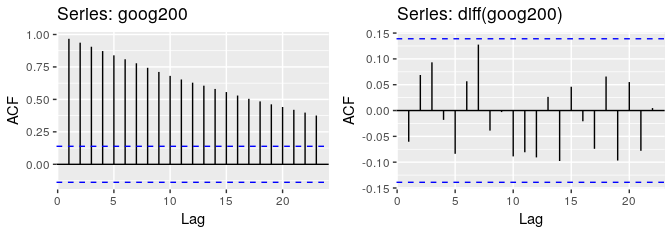
\includegraphics[width=.8\textwidth]{figures/ACF.png}
\caption{The ACF of Google stock prices (left; non-stationary), and its daily price changes (right; stationary). \cite{kdnugget}}
\end{figure}


\begin{theorem}
Some basic properties of the ACVF include:
\begin{enumerate}
    \item $\gamma(0) \geq 0$
    \item $|\gamma(h)| \leq \gamma(0)$ for all $h \in \mathbb{Z}$
    \item $\gamma(h) = \gamma(-h)$ for all $h \in \mathbb{Z}$
\end{enumerate}
\end{theorem}


%\begin{definition}
%    If $x_1, \dots, x_n$ are observations of a time series, then the \textit{sample mean} is defined as
%    \begin{equation*}
%        \bar{x} = \frac{1}{n} \sum^n_{t=1}x_t.
%    \end{equation*}
    
%    The \textit{sample autocovariance function} is
%    \begin{equation*}
%        \hat{\gamma}(h) = \frac{1}{n} \sum^{n-|h|}_{t=1} (x_{t+|h|} - \bar{x})(x_t - \bar{x}),
%    \end{equation*}
    
%    and the \textit{sample autocorrelation function} is
%    \begin{equation*}
%        \hat{\rho}(h) = \frac{\hat{\gamma}(h)}{\hat{\gamma}(0)} \text{ for } -n < h < n.
%    \end{equation*}
%\end{definition}


\section{Estimation and Elimination of Trend and Seasonal Components}\label{sc:trendseason}

This section is based on Section 1.3.3 of \cite{itsf}.

When forecasting time series, we would like to check whether the following things are present:
\begin{enumerate}[label=(\alph*)]
    \item trends
    \item seasonal components
    \item sharp changes in behaviour
    \item outliers.
\end{enumerate}
Ideally, by removing the trend and seasonal components, the residuals i.e. remaining errors should be stationary white noise, meaning that all of the signal information has been analysed already and only random fluctuations remain. If the model predictions are more than just white noise, this signifies that further improvements can be made.

Let us consider the \textit{classical decomposition model}
\begin{equation} \label{eq:classicaldecomp}
    X_t = m_t + s_t + Y_t,
\end{equation}
where $m_t$ is the \textit{trend component} (a more slowly changing function), $s_t$ the \textit{seasonal component} with period $d$, and $Y_t$ being a weakly stationary \textit{noise component}, i.e.
\begin{equation*}
    \E[Y_t] = 0,\quad s_{t+d} = s_t,\text{ and }\sum^d_{j=1}s_j = 0.
\end{equation*}
There are several methods of estimating the trend and seasonality, such as smoothing methods like using a finite moving average filter and exponential smoothing (which we will see in Chapter \ref{chap:exp} in more detail); as well as the differencing methods. For the latter, we shall introduce the difference operators:

\begin{definition}
    The \textit{lag-1 difference operator} $\nabla$ is defined as:
    \begin{equation}
        \nabla X_t = X_t - X_{t-1} = (1-B)X_t.
    \end{equation}
    
    Where the \textit{backward shift operator} $B$ is defined as:
    \begin{equation}
        BX_t = X_{t-1}.
    \end{equation}
    and the \textit{lag-d differencing operator} $\nabla_d$ is defined as
    \begin{equation}
        \nabla_d X_t = (1-B^d) X_t.
    \end{equation}
\end{definition}
\begin{remark}
    Note that $\nabla_d$ is not the same as $\nabla^d$, which is defined as $\nabla^d = (1-B)^d$.
\end{remark}

Differencing a time series $d$ times may result in a stationary time series, allowing us to apply the methods from later chapters which rely on their useful properties.

\section{Estimating the Noise Sequence}\label{sc:noise}

This section is based on Sections 1.4.1 and 1.6 of \cite{itsf}.

Once we have transformed the time series data and isolated the stationary components $Y_t$, the next step is to model the residuals, or “estimated noise sequence”. If these residuals are independent to each other, it remains for us to estimate the mean and variance, and no further action is required. However, if there is a significant level of dependence, we need to consider more complex stationary time series models for the noise. In fact, this is helpful, since dependence between past and present noise terms is beneficial for forecasting future ones.

\subsection{Sample Autocorrelation Method}
We will present one method of testing the residuals, namely the sample autocorrelation function method. Further methods can be found in \cite{itsf}, Section 1.6.

\begin{definition}
    For a time series $\{X_t\}$, the \textit{sample autocovariance function} is defined as
    \begin{equation*}
        \hat{\gamma}(h) = \frac{1}{n} \sum^{n-|h|}_{t=1} (X_{t+|h|} - \bar{X})(X_t - \bar{X}),
    \end{equation*}
    
    and its \textit{sample autocorrelation function} is similarly defined as
    \begin{equation*}
        \hat{\rho}(h) = \frac{\hat{\gamma}(h)}{\hat{\gamma}(0)} \quad \text{for } -n < h < n.
    \end{equation*}
\end{definition}

For $\{X_t\}$ i.i.d. noise, it can be proven that for $n \to \infty$,
\begin{equation*}
    \sqrt{n} \boldsymbol{\hat{\rho}} \xrightarrow{d} N(\mathbf{0}, Id_n) \text{ with } \boldsymbol{\hat{\rho}} := (\hat{\rho}(1), \hat{\rho}(2), \dots, \hat{\rho}(h))^T.
\end{equation*}

Let us now define the quantity
\begin{equation*}
    N_h := \sum_{i=1}^h \mathbbm{1}_{ \{|\hat{\rho}(i)| \geq \frac{Z_{1-\alpha/2}}{\sqrt{n}} \} },
\end{equation*}

where $Z_{1-\alpha/2}$ denotes the $(1-\alpha/2)$th quantile of $N(0,1)$.

It holds $N_h \xrightarrow[]{d} \mathrm{Bin}(h, \alpha)$ as $n \to \infty$, since by ``almost independence'' of $\hat{\rho}(1), \dots, \hat{\rho}(h)$:

\begin{equation*}
    P(|\hat{\rho}(1)| \geq \frac{Z_{1- \alpha/2}}{\sqrt{n}}) \xrightarrow[n\to\infty]{} P(|Z| \geq Z_{1- \alpha/2}) = \alpha.
\end{equation*}

Hence, $\E[N_h] \approx h\alpha$ and $\mathrm{Var}(N_h) \approx h \alpha (1-\alpha)$ for large $n$.

This observation on $N_h$ allows us to perform a hypothesis test on the assumption that the noise is i.i.d.; if it is not the case, then we can expect the number of sample autocorrelations to be larger than $\E[N_h]$.

\begin{figure}[ht]
\centering
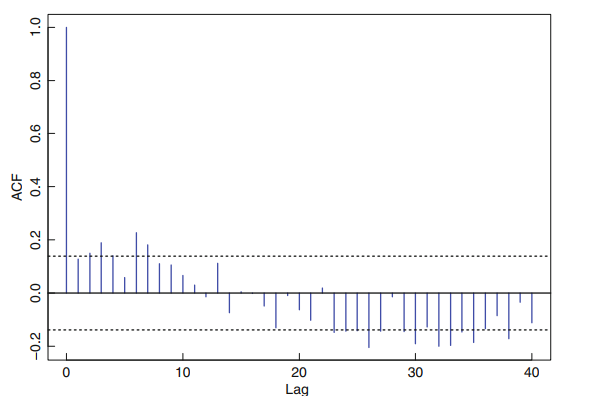
\includegraphics[width=.6\textwidth]{figures/fig1-28.png}
\caption{The sample autocorrelation function for $X_t = \cos{t/10} + N_t$ for $t = 1, \dots, 200$ and $N_t$ a sequence of independent normal variables.(\cite{itsf}, fig. 1-28).}
\end{figure}

\chapter{ARMA Processes}
We will discuss the properties of ARMA processes, conditions showing when the process has a stationary solution, the notion of causality and lastly how to forecast them. As well as being based on Chapters 2, 3 and 5 of \cite{itsf}, some parts of this chapter has been based on \cite{chatfield}.

\textit{Autoregressive moving-average} (ARMA) processes are an important family of models used mainly to model stationary time series. We will see in later sections that they are simple to forecast.
%In particular, for a large class of ACVFs $\gamma(\cdot)$, we can find ARMA processes $\{X_t\}$ whose ACVFs $\gamma_X(\cdot)$ approximate $\gamma(\cdot)$ using algorithms such as Yule-Walker.

We will first begin with a more generalised class of processes (which ARMA itself is a type of) called \textit{linear processes}. These provide us with a framework for analysing stationary processes.

\begin{definition}
    A time series $\{X_t\}$ is a \textit{linear process} if it can be written as
    \begin{equation}
        X_t = \sum_{j=-\infty}^\infty \psi_j Z_{t-j} \quad \forall t,
    \end{equation}
    where $\{Z_t\} \sim \mathrm{WN}(0, \sigma^2)$, and $\{\psi_j\}$ is a real sequence of constants with $\sum_{j=-\infty}^\infty |\psi_j| < \infty$.
\end{definition}

\begin{definition}
    A time series $\{X_t\}$ is said to be an ARMA($p,q$) stationary process if $\{X_t\}$ is stationary, and if for every $t$,
    \begin{equation} \label{eq:2.2}
        \phi(B) X_t = \theta(B) Z_t,
        %X_t - \phi_1 X_{t-1} - \dots - \phi_p X_{t-p} = Z_t + \theta_1 Z_{t-1} + \dots + \theta_q Z_{t-q},
    \end{equation}
    where ${Z_t} \sim \text{WN}(0,\sigma^2)$, the polynomials $\phi(z) = (1-\phi_1z - \dots - \phi_p z^p)$ and $\theta(z) = (1 + \theta_1 z + \dots + \theta_q z^q)$ have no common factors, and $B$ denotes the backward shift operator.
\end{definition}

An ARMA process possesses a \textit{stationary solution} if we can write $X_t$ purely in terms of $Z_t$. This solution can almost surely be unique, as we will see in the theorems below.

\begin{definition}
    A time series $\{X_t\}$ is said to be an \textit{autoregressive process of order $p$} (AR($p$)) if $\theta(z) \equiv 1$, and a \textit{moving-average process of order $q$} (MA($q$)) if $\phi(z) \equiv 1$. An ARMA process is a mixed model, containing $p$ AR terms and $q$ MA terms.
\end{definition}

\section{Causality and Invertibility}

This section is based on Section 3.1 of \cite{itsf}.

ARMA($p,q$) processes can be causal or invertible. These two properties allow us to write a solution of the ARMA($p,q$) process in terms of only past or future values, making it easier to find a solution as well as being able to say more about uniqueness of the solution. Furthermore, causality enables us to conveniently find the ACVF of the ARMA process and shorten the application of the innovations algorithm (see Section \ref{innovations}).

\begin{definition}
    A time series $\{X_t\}$ is a \textit{causal solution} if the linear process can be written as an expression of only current and past values of the white noise term $\{Z_t\}$, i.e.
    \begin{equation} \label{eq:causal}
        X_t = \sum_{j=0}^\infty \psi_j Z_{t-j} \quad \forall t \in \mathbb{Z}.
    \end{equation}
    $\{X_t\}$ is a \textit{non-causal solution} if it can be written only using current and future values of $\{Z_t\}$:
    \begin{equation*}
        X_t = \sum_{j=0}^\infty \psi_j Z_{t+j} \quad \forall t \in \mathbb{Z}.
    \end{equation*}
\end{definition}

A parallel notion to causality is invertibility:

\begin{definition}
    A white noise $\{Z_t\}$ is an \textit{invertible solution} if it can be written as an expression of only current and past values of the time series events $\{X_t\}$:
    \begin{equation*}
        Z_t = \sum_{j=0}^\infty \pi_j X_{t-j} \quad \forall t \in \mathbb{Z}.
    \end{equation*}
    Analogously, a \textit{non-invertible solution} of $\{Z_t\}$ is defined as
    \begin{equation*}
        Z_t = \sum_{j=0}^\infty \pi_j X_{t+j} \quad \forall t \in \mathbb{Z},
    \end{equation*}
    i.e. it can be written purely as present and future values of $X_t$.
\end{definition}

The coefficients $\psi_j$ and $\pi_j$ can be found by Taylor-expanding $1/\phi(z)$ and $1/\theta(z)$ accordingly, in particular, for causal $\{X_t\}$, we can write the coefficients $\psi_j$ as (see \cite{itsf}, section 2.3)

\begin{equation}\label{eq:causal_coeff}
    \psi_j = \theta_j + \sum_{i=1}^{\min(j,p)} \phi_i \psi_{j-i}, \quad j = 0, 1, \dots,
\end{equation}

and we define $\theta_0 := 1$ and $\theta_j := 0$ for $j > q$.

It is important to determine whether a stationary solution of the ARMA equations exists and whether $\{X_t\}$ is causal, which is illustrated in the following theorem.

\begin{theorem}
    If $\phi$ and $\theta$ as defined in \eqref{eq:2.2} do not admit any common factors, then a stationary solution of the equations $\phi(B) X_t = \theta(B) Z_t$ only exists if the AR polynomial $\phi$ does not admit a root on the unit circle.
    
    Furthermore, $\{X_t\}$ is causal if and only if $\phi$ does not admit any roots in the unit disc.
\end{theorem}
This theorem can be proven using properties of the power series, and a proof can be found in the HS20 course "Time Series Analysis" lecture notes (Lecture 11) by F. Balabdaoui.

\section{The ACVF and PACF of ARMA Processes}\label{sc:ACVFPACF}
This section is based on Section 3.2 of \cite{itsf}.
\subsection{ACVF}
\begin{proposition}
    Let $\{Y_t\}$ be a stationary zero-mean time series with covariance function $\gamma_Y$. If $\sum_{j=-\infty}^\infty |\psi_j| < \infty$, then the transformed time series
\begin{equation*}
    X_t = \sum_{j=-\infty}^\infty \psi_j Y_{t-j} = \psi(B) Y_t
\end{equation*}
is itself a stationary zero-mean time series with ACVF
\begin{equation*}
    \gamma_X(h) = \sum_{j=-\infty}^\infty \sum_{k=-\infty}^\infty \psi_j \psi_k \gamma_Y(h+k-j). 
\end{equation*}

Specifically, for a linear process $\{X_t\}$, the above expression is simplified to
\begin{equation} \label{eq:armaacvf}
    \gamma_X(h) = \sum_{j=-\infty}^\infty \psi_j \psi_{j+h} \sigma^2,
\end{equation}
where $\sigma^2$ is the variance of the white noise component $\{Z_t\}$.
\end{proposition}
\begin{proof}
    Cf. p.45 in \cite{itsf}.
\end{proof}

For causal ARMA$(p, q)$ processes
\begin{equation*}
    X_t = \sum_{j=0}^\infty \psi_j Z_{t-j},
\end{equation*}
where $\{\psi_j\}$ is calculated in \cite{itsf}, section 2.3, $\sum_{j=0}^\infty \psi_j z^j = \theta(z)/\phi(z)$, $|z| \leq 1$, there are several ways to calculate their ACVFs $\gamma(h)$. For example, we can use \eqref{eq:armaacvf} to say that $\gamma_X(h) = \sum_{j=0}^\infty \psi_j \psi_{j+|h|} \sigma^2. \label{eq:causalacvf}$ 

The significance of considering the ACVF and ACF respectively lies with the moving-average process $\mathrm{MA}(q)$. From \eqref{eq:armaacvf}, we can deduce, for an $\mathrm{MA}(q)$ process
\begin{equation*}
    X_t = Z_t + \theta_1 Z_{t-1} + \dots + \theta_q Z_{t-q},\quad\{Z_t\} \sim \mathrm{WN}(0, \sigma^2)
\end{equation*}
with ACVF
\begin{equation*}
    \gamma(h) =
    \begin{cases}
        \sigma^2\sum_{j=0}^{q-|h|}\theta_j \theta_{j+|h|}, \quad &\text{if } |h| \leq q, \\
        0, &\text{if } |h| > q,
    \end{cases}
\end{equation*}
where $\theta_0 := 1$, that its ACVF vanishes at $|h| > q$. We can therefore inspect the ACF of a moving average process to see where it is close to $0$. Here, ``close to $0$'' means that the sample ACF values with $h > p$ are approximately distributed as $N(0, 1/n)$ random variables, i.e. they lie within a $95\%$ confidence interval. This property is very useful in order selection of ARMA and even ARIMA models.

\subsection{PACF}
The \textit{partial autocorrelation function} (PACF) $\alpha(\cdot)$ of an ARMA process $\{X_t\}$ is defined by the equations
\begin{equation*}
    \alpha(0) = 1, \quad \alpha(h) = \phi_{hh}, \quad h \geq 1,
\end{equation*}
where $\phi_{hh}$ represents the last component of
\begin{equation*}
    \boldsymbol{\phi}_h = \Gamma_h^{-1} \boldsymbol{\gamma}_h, \quad \gamma_h = [\gamma(i-j)]^h_{i, j=1}, \quad \boldsymbol{\gamma}_h = [\gamma(1), \gamma(2), \dots, \gamma(h)]^T.
\end{equation*}

The \textit{sample PACF} $\hat{\alpha}(h)$ is defined by the relations
\begin{equation*}
    \hat{\alpha}(0) = 1, \quad \hat{\alpha}(h) = \hat{\phi}_{hh}, \quad \boldsymbol{\hat{\gamma}}_h = \hat{\Gamma}_h^{-1} \boldsymbol{\hat{\gamma}}_h.
\end{equation*}

In a similar fashion as to why one considers the ACF and ACVF of an $\mathrm{MA}(q)$ process, it can be shown that, for a purely autoregressive process $\mathrm{AR}(p)$, if the sample PACF $\hat{\alpha}(h)$ is much larger/smaller than $0$ for $0 \leq h \leq p$ and close to $0$ for $h > p$, then an AR$(p)$ model may be a suitable representative of the data (cf. Example 3.2.6 in \cite{itsf}).

\section{Forecasting Stationary Time Series}
This section is based on Section 2.5 of \cite{itsf}.

Forecasting, or extrapolation, involves taking models based on historical data and using them to predict future observations. The future data is completely unavailable and can only be estimated from what has already happened. The effectiveness of a forecasting model is determined by several parameters, such as why a specific prediction was made, underlying relationships, and confidence intervals on how accurate the predictor is compared to actual future values.

\subsection{Derivation of the Linear Prediction Operator}

In order to forecast, we would like to firstly consider the linear prediction operator $P_n$, a special case of the general prediction operator $Y \mapsto P(Y | \boldW)$.

\begin{definition}
    The linear prediction operator $P_n$ is defined as
    \begin{equation} \label{eq:Pn}
        P_n X_{n+h} = a_0 + a_1 X_n + \dots + a_n X_1,
    \end{equation}
    where $a_0, \dots, a_n$ are such that $P_n X_{n+h}$ achieves the smallest prediction error among all such possible linear combinations.
\end{definition}

\begin{theorem}
    The equation \eqref{eq:Pn} can be simplified to
    \begin{equation} \label{eq:2.13}
        P_n X_{n+h} = \mu + \sum_{i=1}^n a_i (X_{n+1-i}-\mu),
    \end{equation}
    where $\mu$ is the mean of the time series.
\end{theorem}

\begin{proof}
This proof follows the derivation from Section 2.5 of \cite{itsf}.

In order to determine the coefficients $a_0, a_1, \dots, a_n$, we would like to find the values that minimise the functional $S$: %\TODO{Do we even need the whole derivation? I feel like it doesn't really contribute to the rest of the paper, and makes the rest of the content confusing} 
\begin{equation*}
    S(a_0, \dots, a_n) = \E[(X_{n+h} - P_n X_{n+h})^2]=\E[(X_{n+h} - a_0 - a_1 X_n - \dots -a_n X_1)^2].
\end{equation*}
To do so, we would like to calculate the partial derivatives of $S$, i.e.
\begin{align}
    \frac{\partial S(a_0, \dots, a_n)}{\partial a_j} &= 0 \\
    \E[X_{n+h} - a_0 - \sum_{i=1}^n a_i X_{n+1-i}] &= 0 \quad j = 0\label{eq:orth1}\\
    \E[(X_{n+h} - a_0 - \sum_{i=1}^n a_i X_{n+1-i})X_{n+1-j}] &= 0 \quad j \geq 1 \label{eq:orth2}
\end{align}
Moreover, we can write the set of equations \eqref{eq:orth2} in vector form:
\begin{equation*}
    a_0 = \mu\left(1-\sum_{i=1}^n a_i\right),
\end{equation*}
and
\begin{equation*}
    \Gamma_n \boldsymbol{a}_n = \boldsymbol{\gamma}_n(h), \label{eq:2.9}
\end{equation*}
where we define
\begin{align*}
    \label{eq:2.10}\boldsymbol{a}_n &= (a_1, \dots, a_n)^T, \\
    \Gamma_n &= [\gamma(i-j)]^n_{i,j=1}, \text{ and}\\ 
    \boldsymbol{\gamma}_n(h) &= (\gamma(h), \gamma(h+1), \dots, \gamma(h+n-1))^T.
\end{align*}
Hence
\begin{equation*} % \label{eq:2.13}
    P_n X_{n+h} = \mu + \sum_{i=1}^n a_i (X_{n+1-i}-\mu)
\end{equation*}
as required.
\end{proof}

\textbf{Properties of $P_nX_{n+h}$}:
\begin{enumerate}
    \item $\E[(X_{n+h} - P_n X_{n+h})^2] = \gamma(0) - \boldsymbol{a}_n^T \boldsymbol{\gamma}_n(h)$.
    \item $\E[X_{n+h} - P_n X_{n+h}] = 0$
    \item $\E[(X_{n+h} - P_n X_{n+h})X_j] = 0$
\end{enumerate}

These properties are equivalent to \eqref{eq:orth1} and \eqref{eq:orth2} and can be referred to as the \textit{orthogonality conditions}.

\subsection{The Prediction Operator and Second-Order Random Variables}
In the more general case, let  $Y$ and $W_n, \dots, W_1$ be arbitrary random variables defined on the same probability space with finite second moments. Let $\mu = \E[Y]$, $\mu_i = \E[W_i]$ and covariances $\Cov(Y,Y)$, $\Cov(Y,W_i)$ and $\Cov(W_j,W_i)$ be all well defined (implied by the finite second moment property). Furthermore, let us denote
\begin{align*}
    \boldW &= (W_n, \dots, W_1)^T, \\
    \boldsymbol{\mu}_W &= (\mu_n, \dots, \mu_1)^T, \\
    \boldsymbol{\gamma} &= \Cov(Y,\boldW) \\
    \boldsymbol{\Gamma} &= [\Cov(W_{n+1-i}, W_{n+1-j})]^n_{j=1}.
\end{align*}
Using an analogous derivation as in the previous section, we obtain that the best linear predictor of $Y$ in terms of $\{1, \dots, w\}$ is given by:
\begin{equation*}
    P(Y | \boldW) = \mu_Y + \boldsymbol{a}^T(W-\mu_W),
\end{equation*}
where $\boldsymbol{a} = (a_1, \dots, a_n)^T$ is defined as a solution of the equation
\begin{equation*}
    \Gamma \boldsymbol{a} = \boldsymbol{\gamma}
\end{equation*}
with mean squared error $\E[(Y-P(Y|\boldW))^2] = \mathrm{Var}(Y) - \boldsymbol{a}^T\boldsymbol{\gamma}$.

\begin{definition}
    For any given $\boldW = (W_n, \dots, W_1)^T$ and $Y$ with finite second moments, the \textit{prediction operator} $Y \mapsto P(Y|\boldW)$ is defined as
    \begin{equation}
        P(Y | \boldW) = \mu_Y + \boldsymbol{a}^T(W-\mu_W).
    \end{equation}
    Letting $\boldW = (X_n, X_{n-1}, \dots, X_1)^T$, we obtain the linear predictor \eqref{eq:2.13}.
\end{definition}

\textbf{Properties of the Prediction Operator $P(\cdot|W)$:} \\
For $U, V$ with finite second moments, $\Gamma = \Cov(\boldW, \boldW)$, and $\beta, \alpha_1, \dots, \alpha_n$ constants, the following facts hold:

\begin{enumerate}
    \item $P(U|\boldW) = \E[U] + \boldsymbol{a}^T(\boldW - \E[\boldW])$, where $\Gamma \boldsymbol{a} = \Cov(U, \boldW).$
    \item $\E[(U - P(U|\boldW))\boldW] = \boldsymbol{0}$, and $\E[(U - P(U|\boldW))] = 0.$
    \item $\E[(U - P(U|\boldW))^2] = \mathrm{Var}(U) - \boldsymbol{a}^T \Cov(U, \boldW).$
    \item $P(\alpha_1 U + \alpha_2 V + \beta | \boldW) = \alpha_1 P(U|\boldW) + \alpha_2 P(V|\boldW) + \beta$.
    \item $P(\sum_{i=1}^n \alpha_i W_i + \beta | \boldW) = \sum_{i=1}^n \alpha_i W_i + \beta$.
    \item If $\Cov(U, \boldW) = \boldsymbol{0}$, then $P(U|\boldW) = \E[U]$.
    \item If $\boldsymbol{V}$ is a random vector such that the components of $\E(\boldsymbol{VV}')$ are all finite, then $P(U|\boldW) = P(P(U|\boldW, \boldsymbol{V})|\boldW)$.
\end{enumerate}

Both the linear and general prediction operators are used extensively in forecasting, such as the innovations algorithm and general forecasting of ARIMA processes. 

\section{The Innovations Algorithm} \label{innovations}
This section is based on Section 2.5.4 of \cite{itsf}.

The innovations algorithm is the de-facto main forecasting algorithm used to predict any time series, regardless of stationarity, and is used in the many popular time series packages, such as \texttt{stats}.

Suppose that $\{X_t\}$ is a zero-mean series with finite second moments for any $t$, and 
\begin{equation*}
    \E[X_iX_j] = \kappa(i,j).
\end{equation*}
Furthermore, let
\begin{equation}
    \label{eq:2.23}\hat{X}_n =
    \begin{cases}
        0, & \text{ if }n = 1, \\
        P_{n-1} X_n, & \text{ if } n \geq 2,
    \end{cases}
\end{equation}
and
\begin{equation*}
    \nu_n = \E[(X_{n+1} - P_nX_{n+1})^2]
\end{equation*}
Lastly, we shall define an \textit{innovation} to be a one-step predictor $U_n := X_n - \hat{X_n}$.

\subsection{The General Innovations Algorithm}

It can be shown that \eqref{eq:2.23} can be rewritten as

\begin{equation}
    \label{eq:innov}\hat{X}_n =
    \begin{cases}
        0, & \text{ if }n = 0, \\
       \sum_{j=1}^n \theta_{nj} U_{n+1-j}, & \text{ if } n \geq 1,
    \end{cases}
\end{equation}
where the coefficients $\theta_{n1}, \dots, \theta_{nn}$ can be recursively computed from the equations
\begin{align}
    \nu_0 &= \kappa(1, 1), \\
    \theta_{n, n-k} &= \nu_k^{-1} \left(\kappa(n+1, k+1) -\sum_{j=0}^{k-1}\theta_{k,k-j}\,\theta_{n, n-j}\,\nu_j\right), \quad 0\leq k <n,
\end{align}
and
\begin{equation}
    \nu_n = \kappa(n+1, k+1) - \sum_{j=0}^{n-1} \theta_{n,n-j}^2\,\nu_j.
\end{equation}
\begin{proof}
    This proof closely follows Proposition 5.2.2 in \cite{tstm}.

    Let $\mathcal{H}_n$ be the closed linear subspace $\mathrm{span}\{X_1, \dots, X_n\}$, and let $\langle X, Y \rangle$ be the scalar product defined by $\E[X, Y]$.
    
    The set $U := \{U_1, U_2, \dots, U_n\}$ is orthogonal w.r.t. $\langle \cdot, \cdot \rangle$, since $U_i \in \mathcal{H}_{j-1}$. Furthermore, $U_j \perp \mathcal{H}_{j-1}$ by definition of $\hat{X}_j$.
    
    Taking the scalar product of both sides of \eqref{eq:2.23} with $U_{k+1}$, $0 \leq k < n$, we have 
    \begin{equation}
        \langle \hat{X}_{n+1}, U_{k+1}\rangle = \theta_{n, n-k}\,\nu_k.
    \end{equation}
    Since $U_{n+1} \perp U_{k+1}$ by orthogonality of $U$, we may apply Gram-Schmidt to calculate the coefficients $\theta_{n, n-k}\,\nu_k$ for $k = 0, \dots, n-1$ as
    \begin{equation}
        \theta_{n, n-k} = \nu_k^{-1} \langle X_{n+1}, U_{k+1}\rangle.
    \end{equation}
    Making use of the representation \eqref{eq:2.23}, and replacing $n$ with $k$, we obtain
    \begin{equation}
         \theta_{n, n-k} = \nu_k^{-1} \left(\kappa(n+1, k+1) - \sum_{j=0}^{k-1} \theta_{k, k-j}\,\theta_{n, n-j}\,\nu_j \right),
    \end{equation}
    as required.
\end{proof}
\newpage
\enlargethispage{3\baselineskip}
\subsection{Application of the Innovations Algorithm to ARMA Processes}
This subsection is based on Section 3.3 of \cite{itsf}.

For causal ARMA processes, we can simplify the Innovations algorithm to
    \begin{equation*}
        \hat{X}_{n+1} = 
        \begin{cases}
            \sum_{j=1}^n \theta_{nj} \left(X_{n+1-j} - \hat{X}_{n+1-j}\right), \quad & 1 \leq n < m, \\
            \phi_1 X_n + \dots + \phi_p X_{n+1-p} + \sum_{j=1}^q \theta_{nj} \left(X_{n+1-j} - \hat{X}_{n+1-j}\right), \quad & n \geq m,
        \end{cases}
    \end{equation*}
where $\theta_{nj}$ can be calculated using the autocovariance $\kappa(i,j)$ (which themselves can be found with \eqref{eq:armaacvf}):
\begin{equation*}
    \kappa(i, j) =
    \begin{cases}
        \sigma^{-2} \gamma_X(i-j), \quad & 1 \leq i, j \leq m, \\
        \sigma^{-2}[\gamma_X(i-j) - \sum_{r=1}^p \phi_r \gamma_X (r-|i-j|)], \quad & \min(i, j) \leq m < \max(i, j) \leq 2m, \\
        \sum_{r=0}^q \theta_r \theta_{r+|i-j|}, \quad & \min(i, j) > m, \\
        0, \quad & \text{otherwise.}
    \end{cases}
\end{equation*}

The mean squared error can be expressed as
\begin{equation} \label{eq:innov_r_n}
    \E[(X_{n+1}-\hat{X}_{n+1})^2] = \sigma^2\E[(W_{n+1}-\hat{W}_{n+1})^2] =: \sigma^2 r_n.
\end{equation}

\begin{proof}
This derivation follows the one in Section 3.3 of \cite{itsf}.

We first consider the transformed time series
\begin{equation} \label{eq:innoarma}
    \begin{cases}
    W_t = \sigma^{-1}X_t, \quad &t = 1, \dots, m, \\
    W_t = \sigma^{-1}\phi(B)X_t, \quad &t > m,
    \end{cases}
\end{equation}
where
\begin{equation}
    m = \max(p,q).
\end{equation}

Without loss of generality, define $\theta_0 := 1$ and $\theta_j:=0$ for $j\leq q$, $p \geq 1$ and $q \geq 1$.

Applying the Innovations Algorithm to $\{W_t\}$ and inferring the coefficients $\theta_{nj}$ the above expression for $\kappa$ gives us
\begin{equation*}
    \begin{cases}
        \hat{W}_{n+1} = \sum_{j=1}^n \theta_{nj} (W_{n+1-j} - \hat{W}_{n+1-j}), \quad & 1 \leq n < m, \\
        \hat{W}_{n+1} = \sum_{j=1}^q \theta_{nj} (W_{n+1-j} - \hat{W}_{n+1-j}), \quad & n \geq m.
    \end{cases}
\end{equation*}
Equations \eqref{eq:innoarma} show us a linear relationship between $X_t$ and its corresponding transformed observation $W_t$. Thus by linearity, the linear one-step predictor $P_n$ is identical for both $W_t$ and $X_t$. We obtain
\begin{equation*}
    \begin{cases}
        \hat{W}_t = \sigma^{-1} \hat{X}_t, \quad & t=1, \dots, m, \\
        \hat{W}_t = \sigma^{-1} [\hat{X}_t - \phi_1 \X_{t-1} - \dots - \phi_p X_{t-p}], & t > m,
    \end{cases}
\end{equation*}
and using \eqref{eq:innoarma} once more, we obtain the required result.
\end{proof}

\begin{corollary}
    The $h$-step predictors satisfy
    \begin{equation}\label{eq:hsteppred}
        P_n X_{n+h} = \sum_{i=1}^p \phi_i P_n X_{n+h-i} + \sum_{j=h}^q \theta_{n+h-1,j}(X_{n+h-j} - \hat{X}_{n+h-j}).
    \end{equation}
\end{corollary}
\begin{proof}
    Cf. Section 3.3.1 in \cite{itsf}.
\end{proof}

\section{Fitting mixed ARMA models using Innovations} \label{chap:mixedARMA}
This section is based on Section 5.1, p.136--137 and Section 5.5.2 of \cite{itsf}.

Prior to forecasting ARMA processes based on our data, we must firstly choose a suitable ARMA process which best fits our data. To this end, we have to determine several parameters, including the choice of $p$ and $q$ (order selection), estimating the mean, the coefficients of $\phi(z)$ and $\theta(z)$, as well as the white noise variance $\sigma^2$. Such methods are implemented in \texttt{forecast}'s \texttt{auto.arima()} function, and this section will only cover such techniques for mixed ARMA models.

\subsection{Estimation of $\phi$ and $\theta$}

Consider a causal model ${X_t}$, which can be expressed using \eqref{eq:causal}, its coefficients $\psi_1, \dots, \psi_{p+q}$ satisfying \eqref{eq:causal_coeff}. To estimate these coefficients, we can refer to the innovation estimates $\hat{\theta}_{m1}, \dots, \hat{\theta}_{m, p+q}$, and substituting these into \eqref{eq:causal_coeff}, we obtain

\begin{equation}\label{eq:causal_innov}
    \hat{\theta}_{mj} = \theta_j + \sum_{i=1}^{\min(j, p)} \phi_i \hat{\theta}_{m, j-i}, \quad j = 1, \dots, p+q.
\end{equation}

We can solve the equations \eqref{eq:causal_innov} by rewriting them in matrix form to get our initial parameter estimates of $\hat{\boldsymbol{\phi}}$ and $\hat{\boldsymbol{\theta}}$:
\begin{equation} \label{eq:causal_innov_mat}
    \begin{pmatrix}
    \hat{\theta}_{m,q+1} \\
    \hat{\theta}_{m,q+2} \\
    \vdots \\
    \hat{\theta}_{m,q+p} \\
\end{pmatrix}
=
\begin{pmatrix}
    \hat{\theta}_{mq} & \hat{\theta}_{m,q-1} & \cdots & \hat{\theta}_{m,q+1-p} \\
    \hat{\theta}_{m,q+1} & \hat{\theta}_{m,q} & \cdots & \hat{\theta}_{m,q+2-p} \\
    \vdots & \vdots & \quad & \vdots \\
    \hat{\theta}_{m,q+p-1} & \hat{\theta}_{m,q+p-2} & \cdots & \hat{\theta}_{m,q} \\ 
\end{pmatrix}
\begin{pmatrix}
    \phi_1 \\
    \phi_2 \\
    \vdots \\
    \phi_p \\
\end{pmatrix}.
\end{equation}

We can now estimate the first $q$ $\theta_j$s using \eqref{eq:causal_innov} and \eqref{eq:causal_innov_mat}:

\begin{equation*}
    \hat{\theta}_{j} = \hat{\theta}_{mj} - \sum_{i=1}^{\min(j, p)} \hat{\phi}_i \, \hat{\theta}_{m, j-i}, \quad j = 1, \dots, q.
\end{equation*}
\newpage
The remaining parameter is the white noise variance $\sigma^2$, which is estimated by
\begin{equation*}
    \hat{\sigma}^2 = \frac{1}{n} \sum_{t=1}^n \left(X_t - \hat{X}_t\right)^2 / r_{t-1},
\end{equation*}
where $\hat{X}_t$ is the one-step predictor calculated using $\hat{\boldsymbol{\phi}}$ and $\hat{\boldsymbol{\theta}}$ from above; $r_n$ is defined as in \eqref{eq:innov_r_n}.

\subsection{Order Selection}

A naive attempt to choose the orders $p$ and $q$ is to set both parameters to be as large as possible. However, this may result in overfitting, meaning that the model may have a low bias (in our case, a low white noise variance) but a higher (test) variance.

We shall turn our attention to some introductory terms:

\begin{definition}
    The \textit{Gaussian Likelihood for an ARMA Process} is defined as
    \begin{equation*}
        L(\boldsymbol{\phi}, \boldsymbol{\theta}, \sigma^2) = \frac{1}{\sqrt{(2\pi \sigma^2)^n r_0 \cdots r_{n-1}}} \exp \left\{-\frac{1}{2\sigma^2} \sum_{j=1}^n \frac{(X_j - \hat{X}_j)^2}{r_{j-1}}\right\}
    \end{equation*}
\end{definition}
(The $r_n$s as well as a motivation of this definition can be found by applying the definition of $\hat{X}_j$ found in the innovations algorithm \eqref{eq:causal_innov})

Following the standard procedure, we differentiate $ L(\boldsymbol{\phi}, \boldsymbol{\theta}, \sigma^2)$ partially w.r.t. $\sigma^2$ and obtain the \textit{maximum likelihood estimators} $\hat{\boldsymbol{\phi}}, \hat{\boldsymbol{\theta}}$ and $\hat{\sigma}^2$:
\begin{align*}
     &S\left(\hat{\boldsymbol{\phi}}, \hat{\boldsymbol{\theta}}\right) = \sum_{j=1}^n \left(X_j - \hat{X}_j\right)^2 / r_{j-1}, \\
     &\hat{\sigma}^2 = \frac{1}{n}S\left(\hat{\boldsymbol{\phi}}, \hat{\boldsymbol{\theta}}\right),
\end{align*}

and $\hat{\boldsymbol{\phi}}, \hat{\boldsymbol{\theta}}$ are the values of $\boldsymbol{\phi}, \boldsymbol{\theta}$ which minimise
\begin{equation*}
     \ell(\boldsymbol{\phi}, \boldsymbol{\theta}) = \ln(n^{-1}  S\left(\boldsymbol{\phi}, \boldsymbol{\theta}\right)) + n^{-1} \sum_{j=1}^n \ln r_{j-1},
\end{equation*}
Using the above terminology, we are able to consider the AICC (Akaike Information [Corrected] Criterion), which is an unbiased estimate of the Kullback-Leibler index :
\begin{definition} The AICC is defined as
    \begin{equation}\label{eq:AICC}
        \mathrm{AICC} := -2 \ln L(\boldsymbol{\phi}_p, \boldsymbol{\theta}_p, S(\boldsymbol{\phi}_p, \boldsymbol{\theta}_p)/n) + 2(p+q+1)n/n(n-p-q-2). 
    \end{equation}
\end{definition}

Minimising this statistic provides us with estimates for $p$ and $q$.


\chapter{ARIMA Processes} \label{chap:ARIMA}
Most time series are not necessarily stationary, hence they cannot be modelled by an ARMA process. However, many can be transformed to an \textit{autoregressive integrated moving-average}, or ARIMA model, which are a generalisation of ARMA processes. The key difference between ARIMA and ARMA is that ARIMA models can also model non-stationary processes; in fact, an ARIMA process reduces to an ARMA process when differenced finitely many times, enabling us to utilise the forecasting methods introduced in the previous chapter.

\section{General ARIMA Processes}
This section is based on Sections 6.1 and 6.4 of \cite{itsf}.
\begin{definition}[ARIMA($p,d,q$) Process]
	A time series $\{X_t\}$ is an \textit{ARIMA($p, d, q$) process} if $Y_t := (1-B)^d X_t$ is a causal ARMA($p, q$) process.
\end{definition}

In particular, $\{X_t\}$ satisfies the difference equation of the form
\begin{equation}
    \label{eq:ARIMA}\phi^*(B)X_t \equiv \phi(B)(1-B)^dX_t = \theta(B)Z_t, \quad \{Z_t\} \sim \mathrm{WN}(0, \sigma^2),
\end{equation}
where $\phi(z) \neq 0$ for $|z| \leq 1$, and the polynomial $\phi^*(z)$ has a zero of order $d$ at $z=1$.

ARIMA processes have the special property that one can add an arbitrary polynomial trend of degree $(d-1)$ to $\{X_t\}$ without altering the difference equation \eqref{eq:ARIMA}, making them especially suited to model processes with trends.

\subsection{Forecasting ARIMA processes}
Let us consider an ARIMA process with $d \geq 1$, since for $d=0$, we can refer to \eqref{eq:2.2}. The first and second moments $\E[X_t]$ and $\E[X_{t+h}X_t]$ cannot be determined by \eqref{eq:ARIMA}, therefore, we require further assumptions to calculate the predictor function. Following an analogous derivation to the linear predictor for ARMA models, we obtain the following expressions for the best ARIMA linear predictor:
\newpage
\begin{theorem}\label{thm:ArimaPred}
    Let $\phi^*(z) = (1-z)^d \phi(z) = 1 - \phi_1^* z - \dots - \phi_{p+d}^* z^{p+d}$ be the ARIMA differencing polynomial. Then for $1 \leq h \leq q$, the best linear predictor for ARIMA processes can be written as
    \begin{equation} \label{eq:hsteppredARIMA}
     P_n X_{n+h} = \sum_{j=1}^{p+d} \phi_j^* P_n Y_{n+h-j} + \sum_{j = h}^q \theta_{n+h-1,j} \, (X_{n+h-j} - \hat{X}_{n+h-j}).
    \end{equation}
    Its mean squared error can be expressed as
    \begin{equation*}
    \sigma_n^2(h) = \E[(X_{n+h} - P_n X_{n+h})^2] = \sum_{j=0}^{h-1}\left(\sum_{r=0}^j \chi_r \theta_{n+h-r-1,j-r}\right)^2 \nu_{n+h-j-1},
    \end{equation*}
    where
    \begin{align*}
        \theta_{n0} &= 1 \\
        \chi(z) &= \sum_{r=0}^\infty \chi_r z^r = (1 - \phi_1^*(z) - \dots - \phi_{p+d}^*(z^{p+d}))^{-1} \\
        \nu_{n+h-j-1} &= \E[(X_{n+h-j} - \hat{X}_{n+h-j})^2] = \E[(Y_{n+h-j} - \hat{Y}_{n+h-j})^2].
    \end{align*}
    By multiplying out terms and comparing coefficients, $\chi_j$ can be found from the recursions
    \begin{equation*}
        \chi_j = \sum_{k=1}^{\min(p,j)} \phi_k^* \chi_{j-k}, \quad j = 1, 2, \dots
    \end{equation*}
    Furthermore, for $h>q$, the general solution, assuming that the AR polynomial $\Phi$ admits distinct roots $(\xi_1, \dots, \xi_p)$, is given by
    \begin{equation}\label{eq:ForecastFunc}
        P_n X_{n+h} = a_0 + a_1h + \dots + a_{d-1}h^{d-1} + b_1\xi_1^{-h} + \dots + b_p \xi_p^{-h} \quad h > q - p - d.
    \end{equation}
\end{theorem}
For the proof, we must consider the following lemmas:
\begin{lemma}\label{lemma1}
    Let $U, W_n, \dots, W_1$ and $\tildeW_n, \dots, \tildeW_1$ be random variables defined on the same probability space such that all of their second moments are finite for all values of $j$. If
    \begin{align*}
        (W_n, \dots, W_1)^T &= \boldsymbol{A}(\tildeW_n, \dots, \tildeW_1)^T  \\
        (\tildeW_n, \dots, \tildeW_1)^T &= \boldsymbol{B}(W_n, \dots, W_1)^T, \quad \boldsymbol{A}, \boldsymbol{B} \in \mathbb{R}^{n\times n},
    \end{align*}
    then 
    \begin{equation*}
        P(U|W_n, \dots, W_1) = P(U|\tildeW_n, \dots, \tildeW_1) \quad \text{almost everywhere.}
    \end{equation*}
\end{lemma}
\newpage
\begin{lemma}
    Let $U, W_n, \dots, W_1$ be as above. Suppose there exists an $i_0 \in \{1, \dots, n-1\}$ such that $\Cov(U, W_{n-j+1}) = 0$ for all $j \in {i_0+1, \dots, n}.$ Then
    \begin{equation*}
        P(U| W_n, \dots, W_1) = P(U | W_n, \dots, W_{n-i_0+1}) \quad \text{almost everywhere.}
    \end{equation*}
\end{lemma}
\begin{proof}
    (of Theorem \ref{thm:ArimaPred}): Assume $\{X_t\}$ satisfies
    \begin{equation*}
        (1-B)^d X_t = Y_t, \quad t = 1, 2, \dots.
    \end{equation*}
    Then by definition, $\{Y_t\}$ is a causal $\mathrm{ARMA}(p,q)$ process and $(X_{1-d}, \dots, X_0)$ is uncorrelated with $Y_t$ for positive $t$. Using the binomial formula, we can rearrange for $X_t$ to obtain
    \begin{equation}\label{eq:3.4}
        X_t = Y_t - \sum_{j=1}^d \binom{d}{j} (-1)^j X_{t-j}, \quad t > 0.
    \end{equation}
    For convenience, we now shift the time scale so that we consider the observations $X_{1-d}, \dots, X_n$, in order to ultimately predict $X_n+h$ based on the past realisations.
    
    By definition of $Y_t$, we observe that $Y_j$ is a linear combination of the past realisations $X_{1-d}, \dots, X_n$. By Lemma \ref{lemma1}, we may apply the best linear predictor operator $P_n$ to both sides of \eqref{eq:3.4} to get
    \begin{equation}\label{eq:3.5}
        P_n X_{n+h} = P_n Y_{n+h} - \sum_{j=1}^d \binom{d}{j} (-1)^j X_{n+h-j}.
    \end{equation}
    Additionally, we may identify $P_n X_{n+1-j} = X_{n+1-j}$, since $X_{n+1-j}$ is itself a linear combination of $X_n, \dots, X_{1-d}$.
    Now let us denote the one-step predictors $P_n X_{n+1} := \hat{X}_{n+1}$ and $P_n Y_{n+1} := \hat{Y}_{n+1}$. Furthermore, we can use \eqref{eq:3.4} and \eqref{eq:3.5} with $h=1$ to obtain 
    \begin{equation*}
        X_{n+1} - \hat{X}_{n+1} = Y_{n+1} - \hat{Y}_{n+1}, \quad n \geq 1.
    \end{equation*}
    Because $\{Y_t\}$ is an ARMA process, we can use \eqref{eq:hsteppred} and the above identity, resulting in
    \begin{equation*}
         P_n X_{n+h} = \sum_{i=1}^p \phi_i P_n Y_{n+h-i} + \sum_{j=h}^q \theta_{n+h-1,j}(X_{n+h-j} - \hat{X}_{n+h-j}).
    \end{equation*}
    Setting $\phi^*(z)$ as in the theorem, we obtain \eqref{eq:hsteppredARIMA} as required.
    
    For $h > q$, \, $\sum_{j=h}^q \theta_{n+h-1,j}\,(X_{n+h-j} - \hat{X}_{n+h-j}) = 0$, and by defining the \textit{forecast function} $g(h) := P_n X_{n+h}$, \eqref{eq:hsteppredARIMA} simplifies down to
    \begin{equation*}
        g(h) = \sum_{j=1}^{p+d} \phi^*_j \, g(h-j) \quad \forall h > q,
    \end{equation*}
    \enlargethispage{\baselineskip}
    and the general solution is given by  \eqref{eq:ForecastFunc} for $h > q - p - d$. The range of $h$ can be explained by observing the smallest argument of $g(h)$ is $h-p-d$.
\end{proof}

    

\section{Seasonal ARIMA Processes}
This section is based on Section 6.5 of \cite{itsf}.

If the data shows signs of seasonality, we have seen from the introduction that it is useful to eliminate the seasonal component of period $s$. A special type of ARIMA process designed to model such processes is the SARIMA process:

\begin{definition} 
    If $d$ and $D$ are non-negative integers, then $\{X_t\}$ is called a \textit{seasonal ARIMA}$(p,d,q)\times(P,D,Q)_s$ \textit{process with period} $s$ if the \textit{differenced} series \\ $Y_t = (1-B)^d (1-B^s)^D X_t$ is a causal ARMA process defined by
    \begin{equation}\label{eq:SARIMA}
        \phi(B) \Phi(B^s) Y_t = \theta(B) \Theta(B^s) Z_t, \quad \{Z_t\} \sim \mathrm{WN}(0, \sigma^2), 
    \end{equation}
    where $\phi(z) = 1 - \phi_1 z - \dots - \phi_p z^p$, $\Phi(z) = 1 - \Phi_1 z - \dots - \Phi_P z^P$, $\theta(z) = 1 + \theta_1 z + \dots + \theta_q z^q$ and $\Theta(z) = 1 + \Theta_1 z + \dots + \Theta_Q z^Q$.
\end{definition}
\begin{remark}
    Analogous to ARMA processes, $\{Y_t\}$ is causal if and only if $\phi(z)$ and $\Phi(z)$ do not possess any roots inside the unit circle. 
\end{remark}

An advantage of using SARIMA models over the classical decomposition model \\ $X_t = m_t + s_t + Y_t$ (cf. Equation \eqref{eq:classicaldecomp}) is that, unlike the classical model which requires the seasonality component $s_t$ to be fixed, SARIMA models allow more flexibility and randomness per cycle, enabling us to simulate a larger class of data. In the practical sense, the parameter $D$ is rarely more than $1$; $P$ and $Q$ are less than $3$.

\section{Forecasting SARIMA Processes}
Forecasting SARIMA processes is similar to its non-seasonal counterpart, except we now obtain the following recursions:

\begin{theorem}
    Let $\{X_t\}$ be a time series fulfilling the equation
    \begin{equation*}
        (1-B)^d (1-B^s)^D X_t = Y_t
    \end{equation*}
    with $d$, $D$ and $s$ as given in \eqref{eq:SARIMA} and $\{Y_t\}$ an ARMA process. Then the best $h$-step linear prediction is given by the recursion
    \begin{equation*}
        P_n X_{n+h} = P_n Y_{n+h} + \sum_{j=1}^{d + Ds} a_j P_n X_{n+h-j}
    \end{equation*}
    with mean squared error
    \begin{equation*}
        \E[(X_{n+h} - P_nX_{n+h})^2] = \sum_{j=0}^{h-1} \left(\sum_{r=0}^j \chi_r \theta_{n+h-r-1, j-r}\right)^2 \nu_{n+h-j-1},
    \end{equation*}
    where $\theta_{nj}$ and $\nu_n$ are calculated using the Innovations Algorithm on $\{Y_t\}$ and
    \begin{equation*}
        \chi(z) = \sum_{r=0}^\infty \chi_r z^r = \frac{1}{\phi(z)\Phi(z^s)(1-z)^d(1-z^s)^D}, \quad |z| < 1.
    \end{equation*}
\end{theorem}

Having covered all the terminology needed to understand SARIMA models and their forcasting methods, we shall turn to another approach of modelling using exponential smoothing.


\chapter{Holt--Winters}
The \textit{Holt--Winters Exponential Smoothing} (HW) or \textit{Triple Exponential Smoothing} method, named after Charles Holt and Peter Winters in 1960, is used for forecasting a time series that shows both a trend and seasonal component. It is based on the three basic notions of smoothing with a finite moving average filter, exponential smoothing, and Holt exponential smoothing. This chapter is based on Sections 1.5 and 10.2 of \cite{itsf}, as well as \cite{little_ts}.

Let us first consider the nonseasonal model of the time series $\{X_t\}$ with trend:
\begin{equation}\label{eq:noseason}
    X_t = m_t + Y_t, \quad t = 1, \dots, n, \quad  \E[Y_t] = 0.
\end{equation}
Let $q$ be a non-negative integer and consider the \textit{two-sided moving average}
\begin{equation*}
    W_t = \frac{1}{2q + 1} \sum_{j=-q}^q X_{t-j} = \frac{1}{2q + 1} \sum_{j=-q}^q m_{t-j} + \frac{1}{2q + 1} \sum_{j=-q}^q Y_{t-j} \approx m_t,
\end{equation*}
under the assumptions that $q+1 \leq t \leq n-q$, the trend $m_t$ is approximately linear over the interval $[t-q, t+q]$ and the average of the error terms are approximately zero over this interval. Then the simple moving average gives us the estimates
\begin{equation*}
    \hat{m_t} = \frac{1}{2q + 1} \sum_{j=-q}^q X_{t-j}, \quad q+1 \leq t \leq n-q.
\end{equation*}
For the cases $t \leq 0$ or $t > n$, packages such as \texttt{stats} define $X_t := X_1$ and $X_t := X_n$ respectively.

Estimation using averaging smooths out the variation of our time series by ``smoothing'' out the variation between points. This method is unreliable due to two reasons: firstly, we consider a two-sided average, meaning that, depending on the value of $t$, we may encounter events in the time series which are in the future; in addition, every historical value is given the same equal emphasis for forecasting future values of the time series which may lead to inaccuracies, leading us to use exponential smoothing.

\section{Exponential smoothing}
Exponential smoothing relies on the assumption that more recent values are more useful to our forecast than the ones further in the past, i.e. the weights of each element of the time series decrease exponentially with respect to time.

Consider again the non-seasonal model denoted by \eqref{eq:noseason}. Then for any fixed $\alpha \in [0, 1]$, the one-sided moving averages $\hat{m}_t$, $t = 1, \dots, n$ are defined by the recursions
    \begin{align}
        \label{eq:exprec1}\hat{m}_t &= \alpha X_t + (1-\alpha) \, \hat{m}_{t-1}, \quad t = 2, \dots, n, \\
        \label{eq:exprec2} \hat{m}_1 &= X_1,
    \end{align}
for some constant $\alpha \in [0,1]$. Substituting \eqref{eq:exprec2} into \eqref{eq:exprec1}, we obtain
    \begin{equation*}
        \hat{m}_t = \sum_{j=0}^{t-2} \alpha (1-\alpha)^j X_{t-j} + (1-\alpha)^{t-1}X_1,
    \end{equation*}
showing the exponentially decreasing weights for $X_t$, especially for $\alpha$ close to $0$, as desired.

As with the naive moving average method, the basic exponential smoothing method is unable to model seasonal models.

\section{Holt's Algorithm}
Let $Y_1, Y_2, \dots, Y_n$ be observations from the non-seasonal model \eqref{eq:noseason}. If the series is stationary, then the slope $m_t$ is constant, and we can express the exponential smoothing $h$-step forecast as
\begin{equation} \label{eq:5.0}
    P_n Y_{n+h} = \hat{m}_n.
\end{equation}
However, for data which is not necessarily stationary, i.e. its trend is not constant, we can generalise the above expression and obtain
\begin{equation}\label{eq:5.1}
	P_n Y_{n+h} = \hat{a}_n + \hat{b}_n h, \quad h = 1, 2, \dots ,
\end{equation}
where $\hat{a}_n$ and $\hat{b}_n$ are denoted as the estimates of the ``level'' and ``slope'' of the trend $\hat{m}_n$, respectively.

Let us denote the one-step forecast $P_n Y_{n+1}$ as $Y_{n+1}$. From \eqref{eq:5.1} and setting $h=1$, we obtain
\begin{equation}\label{eq:5.2}
	\hat{Y}_{n+1} = \hat{a}_n + \hat{b}_n.
\end{equation}
\newpage
Holt's algorithm estimates $\hat{a}_n$ and $\hat{b}_n$ in a similar recursive fashion to the exponential smoothing method as
\begin{align}
	\hat{a}_{n+1} &= \alpha Y_{n+1} + (1-\alpha)(\hat{a}_n + \hat{b}_n), \label{eq:5.3} \\
	\hat{b}_{n+1} &= \beta(\hat{a}_{n+1} - \hat{a}_n) + (1-\beta)\hat{b}_n, \label{eq:5.4}
\end{align}
with initial conditions
\begin{equation*}
    \hat{a}_2 = Y_2, \quad \hat{b}_2 = Y_2 - Y_1.
\end{equation*}
Equations \eqref{eq:5.3} and \eqref{eq:5.4} make use of the exponential smoothing parameters $\alpha$ and $\beta$ similar to \eqref{eq:exprec1}. These are best chosen between $0$ and $1$ to minimise the MSE \\ $\sum_{i=3}^n (Y_i - P_{i-1} Y_i)^2$.

Now we would like to show that Holt's algorithm is analogous to ARIMA. Using \eqref{eq:exprec1} and \eqref{eq:5.0}, the one-step forecasts obtained by exponential smoothing with parameter $\alpha$ can be re-written as:
\begin{equation}
    P_nY_{n+1} = Y_n - (1-\alpha)(Y_n - P_{n-1}Y_n), \quad n \geq 2
\end{equation}
Notice that these are the same relations satisfied by the large-sample minimum MSE forecasts of the invertible $\mathrm{ARIMA}(0,d,q)$ process
\begin{equation} \label{eq:5.8}
    Y_t = Y_{t-1} + Z_t - (1-\alpha) Z_{t-1}, \quad \{Z_t\} \sim \mathrm{WN}(0, \sigma^2),
\end{equation}
with optimised $\alpha$ found by minimising the average squared error of the one-step average squared error.

In the general case, it can be shown that Holt's Algorithm can be viewed as fitting a family of $\mathrm{ARIMA}(p,d,q)$ processes
\begin{equation}\label{eq:5.9}
    (1-B)^2Y_t = Z_t - (2 - \alpha - \alpha \beta) Z_{t-1} + (1-\alpha) Z_{t-2}, \quad \{Z_t\} \sim \mathrm{WN}(0, \sigma^2).
\end{equation}
The coefficients $\alpha$ and $\beta$ are selected as described above, and the estimate of $\sigma^2$ is the average squared error of the one-step forecasts of $Y_3, \dots, Y_n$ obtained using the methods described in Chapter \ref{chap:mixedARMA}.


\section{Holt--Winters' Algorithm}
The methods described in the previous section were based on the non-seasonal model assumption \eqref{eq:exprec1}. However, data such as that used in Chapter \ref{chap:exp} is expected to possess seasonality, hence we need to expand on Holt's Algorithm. In essence, we now consider three parameters $\alpha$, $\beta$ and $\gamma$, where $\gamma$ now models the seasonal component at the current point in time. Generalising the $h$-step forecast again, we obtain
\begin{equation}\label{eq:HW}
    P_n Y_{n+h} = \hat{a}_n + \hat{b}_n h + \hat{c}_{n+h}, \quad h=1, 2, \dots,
\end{equation}
where $\hat{c}_{n+h}$ represents the seasonal component. Letting $k$ be the smallest integer such that $n+h-kd \leq n$, then we set the $\hat{c}_i$s to have a seasonal structure:
\begin{equation*}
    \hat{c}_{n+h} = \hat{c}_{n+h-kd}, \quad h=1, 2, \dots,
\end{equation*}
and similar to \eqref{eq:5.3} and \eqref{eq:5.4}, we obtain the three following recursions for $\hat{a}_i$, $\hat{b}_i$ and $\hat{c}_i$ (leading to the procedure's alternative name of triple exponential smoothing):
\begin{align*}
    \hat{a}_{n+1} &= \alpha\, (Y_{n+1} - \hat{c}_{n+1-d}) + (1-\alpha)(\hat{a}_n + \hat{b}_n), \\
    \hat{b}_{n+1} &= \beta\, (\hat{a}_{n+1} - \hat{a}_n) + (1-\beta)\,\hat{b}_n, \\
    \hat{c}_{n+1} &= \gamma\, (Y_{n+1} - \hat{a}_{n+1}) + (1-\gamma)\,\hat{c}_{n+1-d},
\end{align*}
with initial conditions
\begin{align*}
    \hat{a}_{d+1} &= Y_{d+1}, \\
    \hat{b}_{d+1} &= (Y_{d+1}- Y_1) /d, \\
    \hat{c}_i &= Y_i - (Y_1 + \hat{b}_{d+1}(i-1)), \quad i = 1, \dots, d+1.
\end{align*}
As with Holt' algorithm, we can specify the smoothing parameters $\alpha$, $\beta$ and $\gamma$ to have values between $0$ and $1$, optimised to minimise the MSE $\sum_{i=d+2}^n(Y_i - P_{i-1}Y_i)^2$. Furthermore, we can again find an analogy between Holt--Winters and ARIMA. It can be proven that the recursions \eqref{eq:HW} are equivalent to the ARIMA forecasts
\begin{align*}
    (1-B)(1-B^d)Y_t = Z_t &+ \dots + Z_{t-d+1}  \\ &+\gamma(1-\alpha)(Z_{t-d}-Z_{t-d-1}) - (2-\alpha -\alpha\beta)(Z_{t-1} +\dots + Z_{t-d}) \\
    &+ (1-\alpha)(Z_{t-2} + \dots + Z_{t-d-1}).
\end{align*}
Naturally, the question arises as to what the difference between seasonal ARIMA and Holt--Winters is and which one performs better. We will discuss the advantages and disadvantages of both methods in the following chapter, as well as compare their effectiveness in forecasting on the Swiss deaths dataset. 


\chapter{Experiments} \label{chap:exp}
%A part of this chapter is inspired by \cite{itsmr_git}.
Having investigated the theory behind the different approaches to time series forecasting, we shall now perform some numerical experiments. All methods were implemented in \texttt{R} and applied to the Swiss Weekly deaths (65+) datasets \cite{deaths_2010-2019} \cite{deaths_2020-2021}.


The \texttt{R} packages \texttt{stats} and \texttt{forecast} contain the methods \texttt{ARIMA()}, \texttt{auto.arima()} and \texttt{HoltWinters()} will be used to perform the required analysis. Furthermore, the \texttt{forecast} package contains useful methods such as \texttt{ggtsdisplay()}, \texttt{checkresiduals()} and \texttt{autoplot()}, aiding us with the visualisation of our analysis. The code for each method can be found in Chapter \ref{chap:Code}.

Firstly, we will train  both models on the deaths dataset from 2010 to 2018, and will attempt to forecast 52 weeks ahead, verifying our forecasting using the testing set data for 2019.

Observing the figure below, we already notice a clear pattern of seasonality in our data towards the end and beginning of each year. This corresponds to the hypothesis that many elderly are more prone to illnesses in winter, such as the flu.

\begin{figure}[H]
\centering
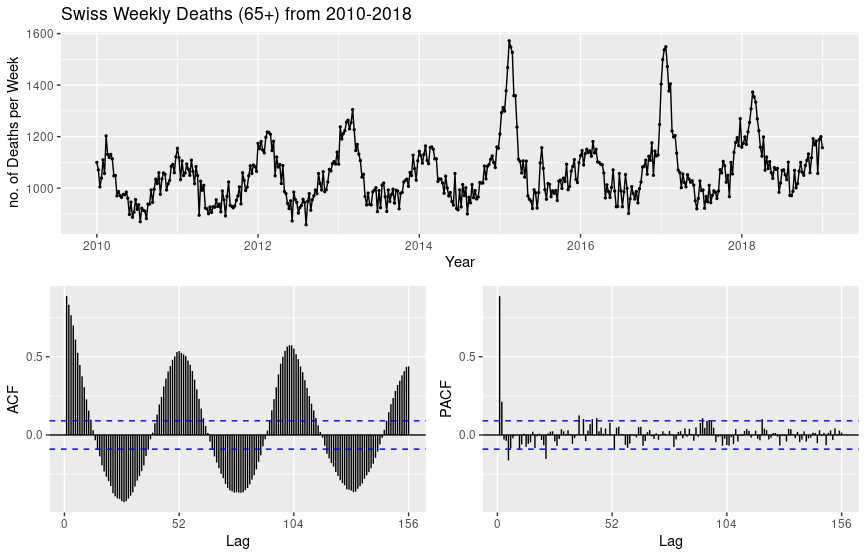
\includegraphics[width=.8\textwidth]{figures/ts_10_18.png}
\caption{Swiss Deaths 65+ Time Series, ACF and PACF from 2010-2018 \cite{deaths_2010-2019}}
\label{fig:ts_10_18}
\end{figure}


\section{SARIMA}
We follow a similar procedure to Example 6.5.4 in \cite{itsf}, Section 2.6 in \cite{little_ts} and Section 8.9 of \cite{fpp2}.

Reiterating the theory from the previous chapters, the methodology of manually forecasting SARIMA processes is as follows:
\begin{enumerate}
    \item Transform the dataset until we obtain a stationary time series. This is done using the methods described in Section \ref{sc:trendseason}.
    \item Plot the modified, now stationary time series' PACF and ACF and note any spikes and their lags. This provides us with our estimates of the ARMA coefficients $p$ and $q$. (cf. Section \ref{sc:ACVFPACF})
    \item Fit an ARMA model using the innovations algorithm (cf. Chapter \ref{chap:mixedARMA}) and calculate the residuals and note the AICC and RMSE (root MSE). Test the noise using the methods from Section \ref{sc:noise}.
    \item Inspect the ACF again and adjust the parameters $p$ and $q$ and adjust accordingly.
\end{enumerate}

By analysing figure \ref{fig:ts_10_18}, we see that the ACF of our dataset is sinusoidal in form and outside of the confidence region, and there is a large spike in the PACF near 0 which then tails off to $0$, indicating that the series can be made stationary after differencing. Furthermore, we would like to have a zero-mean time series, so we shall difference the data once to obtain the following graphic:
\begin{figure}[H]
\centering
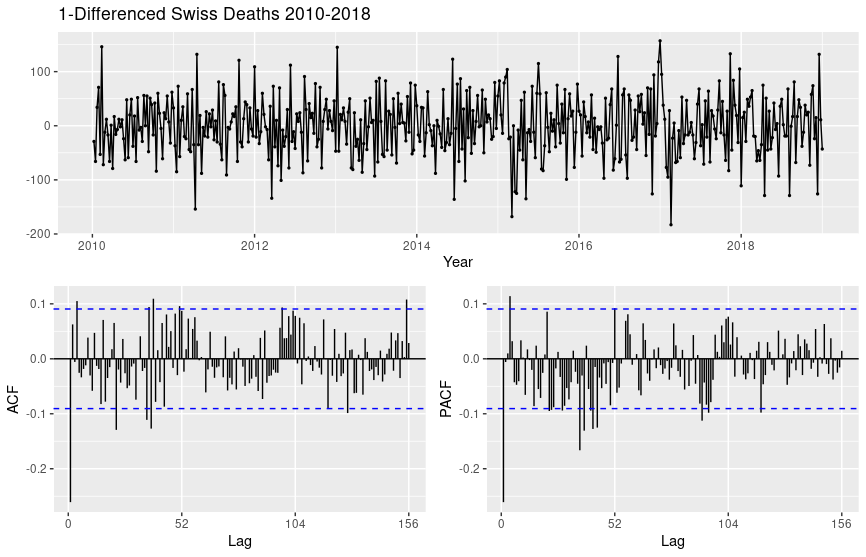
\includegraphics[width=.8\textwidth]{figures/ts_10_18_diff.png}
\caption{1-Differenced Swiss Deaths 2010-2018}
\end{figure}
\newpage
The differenced time series appears to be more stationary and well behaved around a common mean $0$, its ACF and PACF also much better behaved, with both functions tailing off to $0$ for larger lags, and the ACF only showing a significant spike at lag $=50\approx1$ year. This implies that a good estimate for an ARIMA model is SARIMA$(0,1,1)\times(0,1,1)$.

After making this initial guess, we attempt to fit the SARIMA$(0,1,1)\times(0,1,1)$ model to our data, and obtain the following results:

\verbfilenobox{data/output_arima_init.txt}

i.e. our time series is estimated to have the form $Y_t = (1 - 0.3984B)(1 - B^{52})Z_t$, $Z_t \sim \mathrm{WN}(0, 2436)$.

Plotting the residuals for the inital guess, we see that the noise is a white noise around $0$ with standard deviation $\sqrt{2436} \approx 49$. Furthermore, the ACF is within the appropriate confidence levels save a few small spikes. However, the large spike in the histogram at level $0$ suggests that the distribution may not be normal. To check this, we perform a Shapiro-Wilk test at a significance level of $5\%$ to check for normality \cite{shapirowilk}. This produces a p-value of $6.623\times 10^{-5} \ll 0.05$, hence we can only deduce that the residuals follow a white noise distribution.

\begin{figure}[H]
\centering
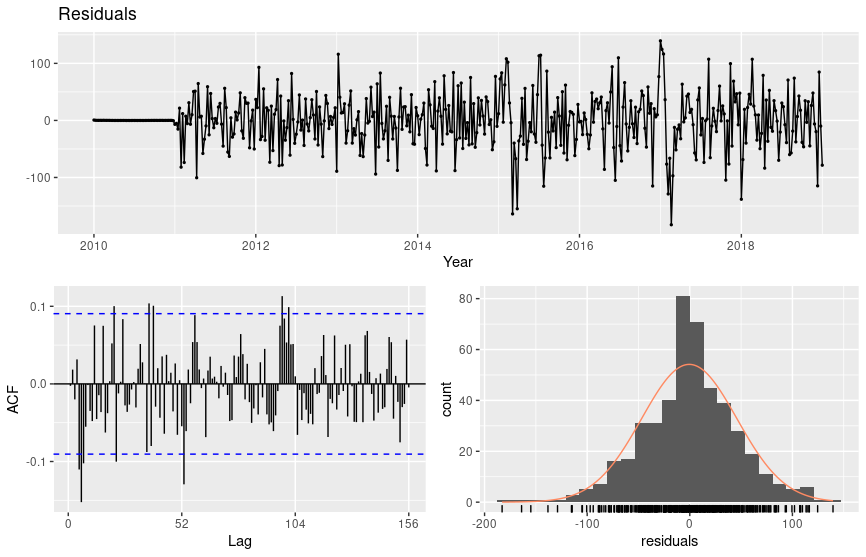
\includegraphics[width=.75\textwidth]{figures/arima_init_resid_acf.png}
\caption{Initial Seasonal ARIMA Model Residuals, ACF, and Initial Seasonal ARIMA Residual Histogram, showing a white noise distribution with mean $0$ and stdev. $\approx 49$}
\end{figure}

Using the \texttt{forecast} function, we obtain the forecast below.
\begin{figure}[H]
\centering
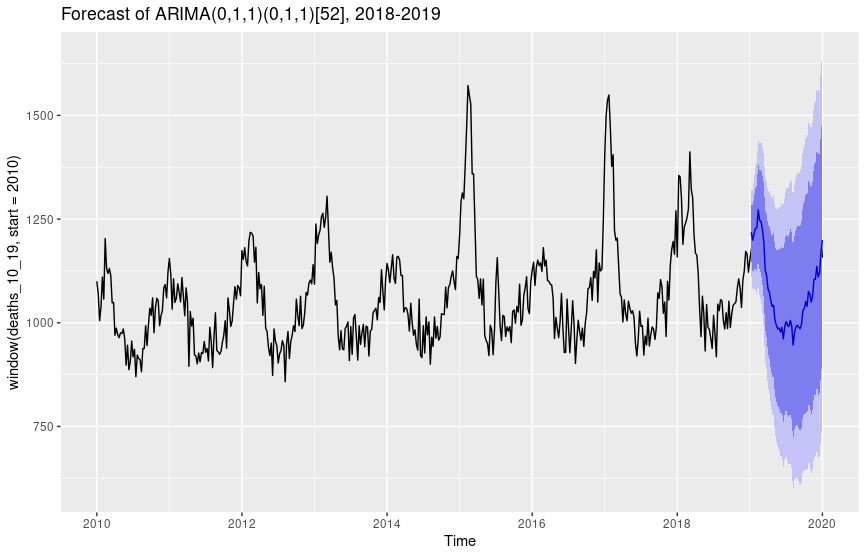
\includegraphics[width=.8\textwidth]{figures/arima_init_forecast.png}
\caption{Initial Seasonal ARIMA Forecasts. The dark blue confidence region represents the 80\% percentile, light blue represents the 95\% percentile.}
\end{figure}
Comparing with the actual testing data, we obtain the following errors:
\verbfilenobox[\scriptsize]{data/accuracy_ar_init.txt}
We are only interested in the RMSE (root mean squared error), and we will compare each method's error in the comparison section.

The \texttt{forecast} package also contains the \texttt{auto.arima()} function, providing us with automatic estimates of the orders of our seasonal model as well as estimates for each of the autoregressive and moving average coefficients. Running \texttt{auto.arima()} gives us the following output:
\verbfilenobox{data/output_arima_auto.txt}
i.e.
\begin{equation*}
    (1-0.6625B)(1+0.5517B^{52})(Y_t-a-bt) = Z_t, \quad Z_t \sim \mathrm{WN}(0, 3464), \quad a, b \in \mathbb{R}
\end{equation*}
where drift represents a fitted linear regression with ARIMA errors, i.e. we replace $Y_t$ with $(Y_t-a-bt)$. (The theory behind ARIMA drifts is outside the scope of this thesis, however additional information can be found in \cite{drift_R} and \cite{drift}). Surprisingly, the automatic ARIMA model produces larger values of the AIC and AICc compared to the initial guess, suggesting that \texttt{auto.arima} did not search all possible models. Adding the parameters \texttt{stepwise=FALSE} and \texttt{approximation=FALSE} forces the algorithm to check more possiblities, however, the code did not stop executing upon multiple tries.

As with the initial guess, we plot the model's residuals and note that the ACF and PACF both show lags at weeks $52$ and $104$, i.e. $1$ and $2$ years, showing that the automatically chosen model can be improved on. Performing a Shapiro--Wilk test at a $5\%$ significance level produces a p-value of $0.004941 \ll 0.05$, so we again deduce that the residuals maintain a zero-mean white noise distribution with standard deviation $\sigma = \sqrt{3464} \approx 59$.
\begin{figure}[H]
\centering
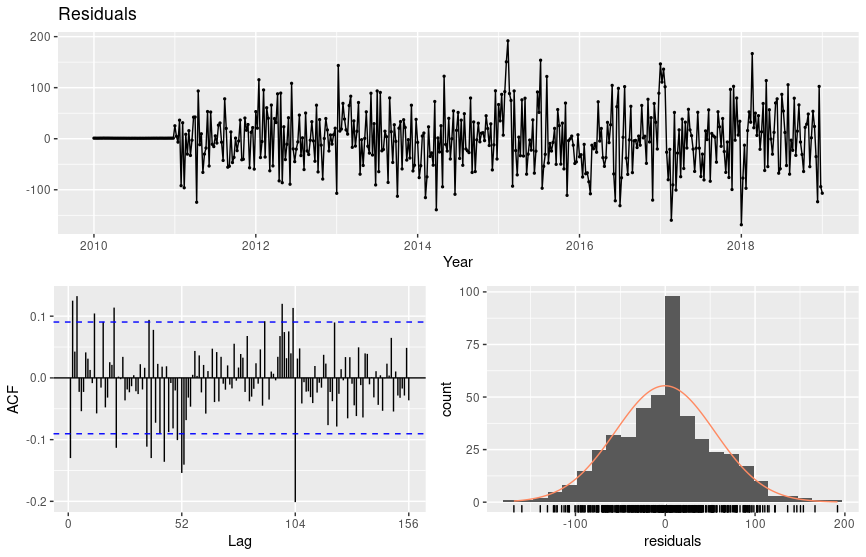
\includegraphics[width=.8\textwidth]{figures/arima_auto_resid_acf.png}
\caption{Automatic Seasonal ARIMA Residuals, ACF, and automatic Seasonal ARIMA residual Histogram, showing a white noise distribution with mean $0$ and stdev. $\approx 59$}
\end{figure}
\begin{figure}[H]
\centering
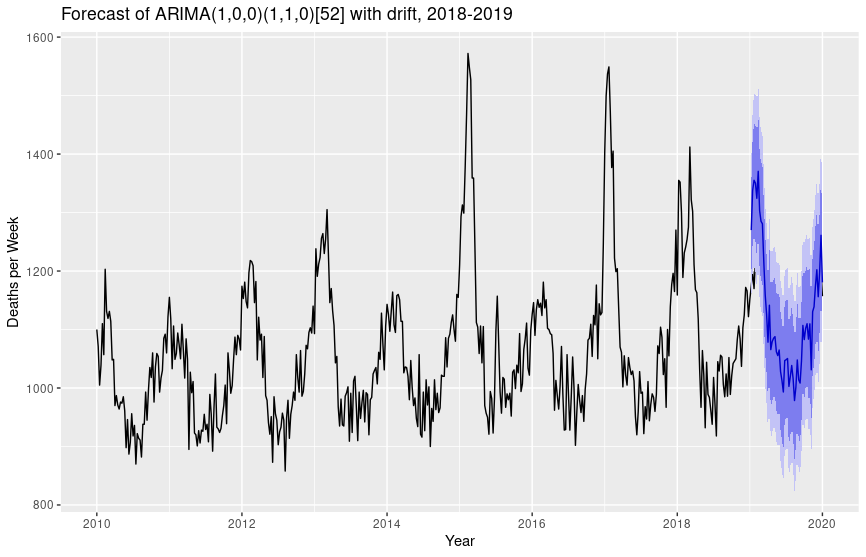
\includegraphics[width=.8\textwidth]{figures/arima_auto_forecast.png}
\caption{Automatic Seasonal ARIMA Forecast. The dark blue confidence region represents the 80\% percentile, light blue represents the 95\% percentile.}
\end{figure}
The forecast above produces the following errors:
\verbfilenobox[\scriptsize]{data/accuracy_ar_auto.txt}
Notice that the RMSE is on average smaller in the initial guess, however the RMSE in the automatic model stays more consistent between the training set and test set, showing less overfitting to our data.


\section{Holt--Winters}
As with seasonal ARIMA, we shall follow a similar route to \cite{itsf} as well as the article \cite{little_ts}.

We first begin by fitting a Holt--Winters model to the deaths dataset from 2010-2018, noting that we leave the rest of the inputs of \texttt{HoltWinters()} blank to indicate that we want to model a possible trend and seasonality. Running the model provides us with the following Holt--Winters estimates for $\alpha$, $\beta$ and $\gamma$:
\verbfilenobox[\small]{data/output_hw.txt}
with $\beta = 0$, since our data shows no visible trend.

Plotting the Holt--Winters estimates for the training data, we observe a visible smoothing of the data, as its alternative name \textit{Triple Exponential Smoothing} suggests.
\begin{figure}[H]
\centering
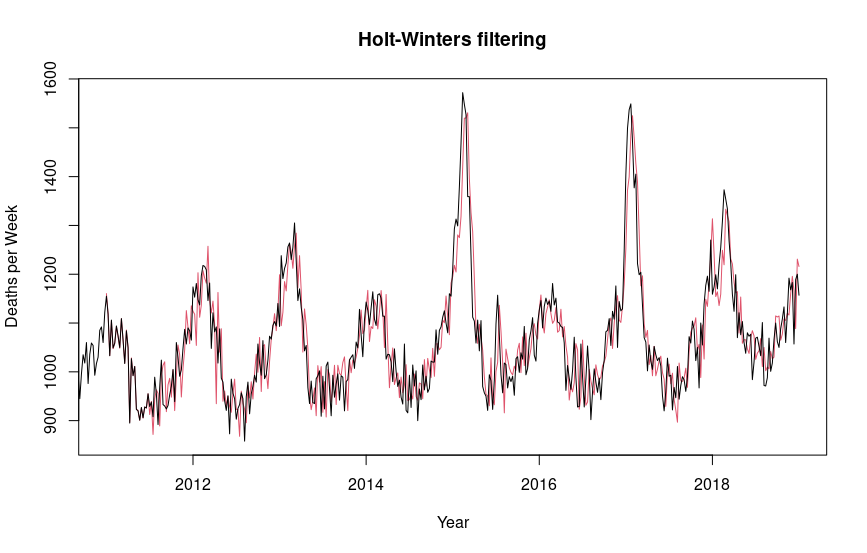
\includegraphics[width=.77\textwidth]{figures/hw_smoothed.png}
\caption{Smoothed Prediction on Training Data from 2010-2018}
\end{figure}
Following the same procedure to the SARIMA models, we plot the the residuals, their histogram and the ACF and note that there are no major spikes in the ACF, unlike the SARIMA family, suggesting a more stable model. The histogram peak at $0$ is less significant than the SARIMA models, and performing a Shapiro--Wilk test at a $95\%$ significance level produces the p-value $0.05066$, showing that the Holt--Winters residuals follow a Gaussian distribution.
\begin{figure}[H]
\centering
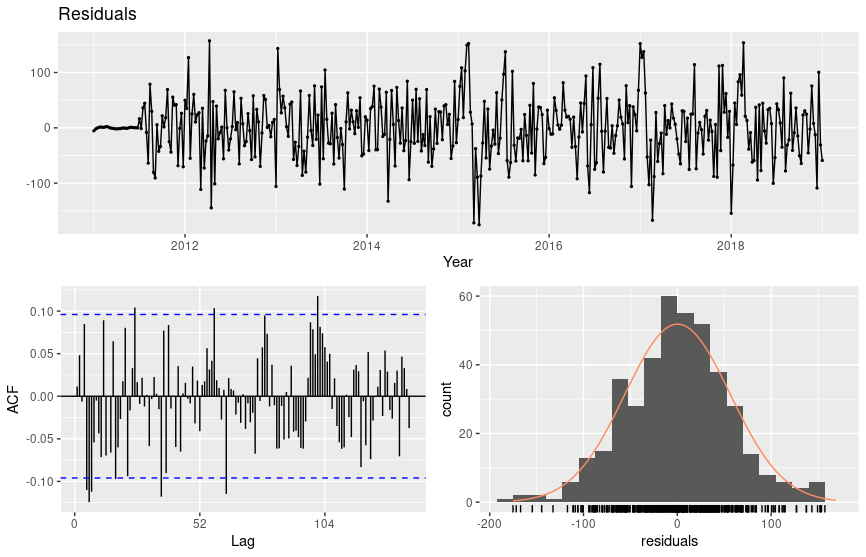
\includegraphics[width=.77\textwidth]{figures/hw_resid_acf.png}
\caption{Holt--Winters Residuals, ACF, and residual histogram, showing a normal distribution.}
\end{figure}

Plotting the forecast, we notice a more modest peak compared to the ones forecasted by the SARIMA models. We also observe that the confidence regions are tighter than the previous two models.
\begin{figure}[H]
\centering
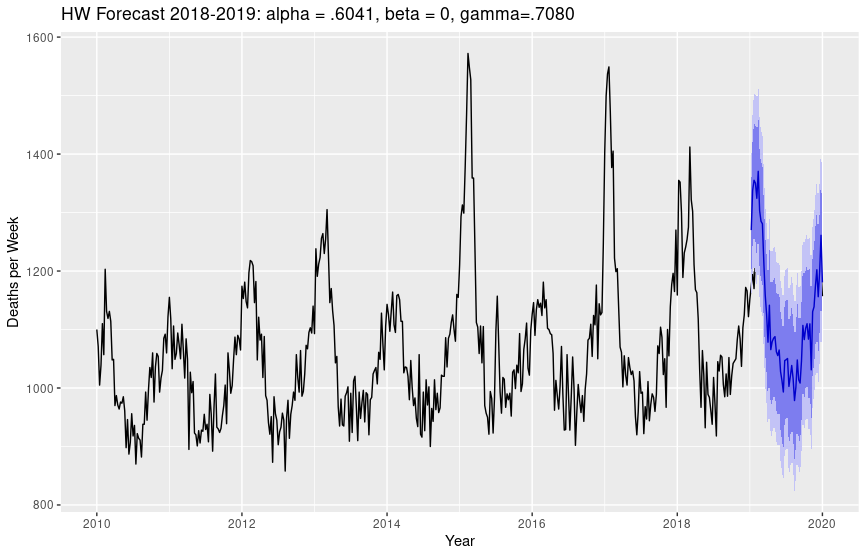
\includegraphics[width=.83\textwidth]{figures/hw_forecast.png}
\caption{Holt--Winters Forecast. The dark blue confidence region represents the 80\% percentile, light blue represents the 95\% percentile.}
\end{figure}
The RMSE for the Holt--Winters forecast are as follows:
\verbfilenobox[\scriptsize]{data/accuracy_hw.txt} showing that the model here performs the worst in both the training and testing sets.
\newpage
\section{Comparison}
We now compare the three models seen in the previous sections and analyse their differences.
\begin{figure}[H]
\centering
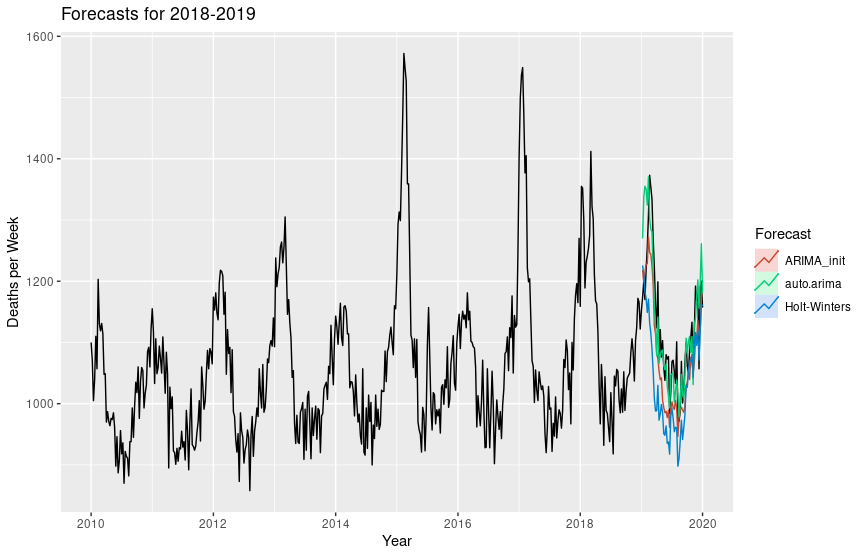
\includegraphics[width=.9\textwidth]{figures/all_2019.png}
\caption{Comparison of all three methods, forecast from 2018-2019}
\end{figure}
\verbfilenobox{data/accuracies.txt}
The automatically determined seasonal ARIMA model performs the best, with the Holt--Winters forecast performing the poorest.

We can also use the data collected from 2010 to 2019 to produce a second forecast for 2020, following an analogous procedure to above:
\begin{figure}[H]
\centering
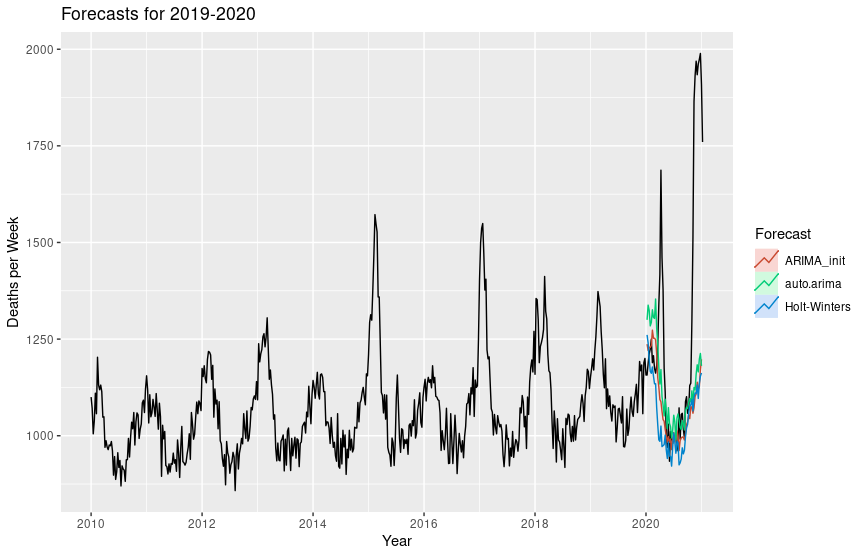
\includegraphics[width=.9\textwidth]{figures/all_2020.png}
\caption{Comparison of all three methods, forecast from 2019-2020}
\end{figure}
Since all three models are based on a seasonal assumption, none of the models could successfully emulate the surge in deaths in the elderly caused by COVID-19.

\section{Conclusion and Outlook}
All three methods provide us with a good forecast for the Swiss deaths dataset from 2018-2019. However, real data is not always generated by a relatively simple model such as a seasonal ARIMA process. Furthermore, using the RMSE may not be the best indication of whether a model is accurate or not, and even within the scope of viewing the RMSE, we could also pose the question of whether we should minimise the one-step, two-step, or in our case, the $52$-step MSE (p.319, \cite{itsf}).

More complicated algorithms, such as Holt--Winters, are likely to be more flexible in practical forecasting problems. However, deciding which models to use is not inherently clear without performing the forecasts and comparing their respective errors.

Nonetheless, none of the models explored in this thesis were able to forecast the drastic change in deaths in 2020. Additional methods, such as choosing methods more suited towards epidemiology like the SIR model and adding parameters related to the reproduction number can be explored, and is beyond the scope of this thesis.

\newpage 

\bibliographystyle{IEEEtran}
\bibliography{references}


%\begin{thebibliography}{9}
%\end{thebibliography}

% This creates an appendix chapter, comment if not needed.
\appendix
\chapter{Code} \label{chap:Code}
The code used in Chapter \ref{chap:exp} can be found here, and is loosely based on the procedures explored in \cite{fpp2} and \cite{little_ts}. All files can also be found under the github repository at \url{https://github.com/wayne-zeng/time-series-forecasting}. In case the links to the Swiss Federal Health Department do not work anymore, csv files from March 2021 are also included in the repository. 

The function \texttt{checkresiduals()} from the library \texttt{forecast} plots a histogram of the forecast errors with an overlaid normal curve that has mean zero and the same standard deviation as the distribution of forecast errors.

\section{Utilities}
\lstinputlisting[language=R, caption=Utility file used for later code]{code/util.R}
\section{SARIMA}
\lstinputlisting[language=R, caption=Script used to generate seasonal ARIMA model forecasts]{code/ARIMA.R}
\section{Holt--Winters}
\lstinputlisting[language=R, 
caption=Holt Winters Method
]{code/HoltWinters.R}
\section{Comparisons}
\lstinputlisting[language=R, 
caption=comparison of all three models
]{code/comparison.R}

\chapter{ARAR Method}

The ARAR algorithm is an adapted version of the ARARMA algorithm, in which the idea is to apply automatically selected “memory-shortening” transformations (if necessary) to the data and then to fit an ARMA model to the transformed series. The ARAR algorithm we describe is a version of this in which the ARMA fitting step is replaced by the fitting of a subset AR model to the transformed data. More information can be found in Section 10.1 of \cite{itsf} as well as \cite{ararma}

This algorithm was originally considered for the thesis. However, the package \texttt{itsmr} used is outdated, provide very little flexibility. The frequency of the time series cannot be specified, unlike \texttt{forecast}, and the ARAR model was not able to produce any significant forecasts.

%\section{Memory Shortening}
%Given a data set $\{Y_t, t = 1, 2, \dots, n\}$, the first step is to decide whether the underlying process is "long-memory", and if so to apply a memory-shortening transformation before attempting to fit an autoregressive model. There are two types allowed:

%\begin{equation} \label{eq:4.1}
%    \Tilde{Y}_t = Y_t - \hat{\phi}(\hat{\tau}) Y_{t-\hat{\tau}} 
%\end{equation}

% and

% \begin{equation} \label{eq:4.2}
%     \Tilde{Y}_t = Y_t - \hat{\phi}_1 Y_{t-1} - \hat{\phi}_2 Y_{t-2}.
% \end{equation}

% We would like to apply the algorithm below to classify $\{Y_t\}$ and declare it to be one of three types of memory:

% \begin{itemize}
%     \item \textbf{L.} Declare $\{Y_t\}$ to be \textit{long-memory} and form $\{\Tilde{Y}_t\}$ using \eqref{eq:4.1}.
%     \item \textbf{M.} Declare $\{Y_t\}$ to be \textit{moderately long-memory} and form $\{\Tilde{Y}_t\}$ using \eqref{eq:4.2}.
%     \item \textbf{S.} Declare $\{Y_t\}$ to be \textit{short-memory}.
% \end{itemize}

% If class L or M is chosen, then the transformed series $\{\Tilde{Y}_t\}$ is again checked. If it is found to be long-memory or moderately long-memory, then a further transformation is performed. The process is continued until the transformed series is classified as short- memory. At most three memory-shortening transformations are performed, but it is uncommon to require more than two. We can classify L, M and S using the following algorithm:

% \begin{algorithm}[H]
% %\SetAlgoLined
% \KwResult{Classifies $\{Y_t\}$ as either S, M, or L memory type}
%  initialization\;
%  \For{$\tau = 1, 2, \dots, 15$}{
%     find value $\hat{\phi}(\tau)$ of $\phi$ that minimises:
%     \begin{equation}
%         \mathrm{ERR}(\phi, \tau) = \frac{\sum_{t=\tau + 1}^n [Y_t - \phi Y_{t-\tau}]^2}{\sum_{t=\tau+1}^n Y_t^2}\;
%     \end{equation}
%     We further define
%     \begin{equation}
%         \mathrm{Err}(\tau) = \mathrm{ERR}(\hat{\phi}(\tau), \tau)
%     \end{equation}
%     and choose the lag $\hat{\tau}$ to be the value of $\tau$ which minimises $\mathrm{Err}(\tau)$\;
%     \uIf{$\mathrm{Err}(\hat{\tau}) \leq 8/n$}{
%         Classify $\{Y_t\}$ as L.\;
%     }
%     \uElseIf{$\hat{\phi}(\hat{\tau}) \geq 0.93$ and $\tau > 2$}{
%         Classify $\{Y_t\}$ as L. \;
%     }
%     \uElseIf{$\hat{\phi}(\hat{\tau}) \geq 0.93$ and $\tau = 1$ or $2$}{
%         Minimise $\sum_{t=3}^n[Y_t - \phi_1 Y_{t-1} - \phi_2 Y_{t-2}]^2$\;
%         Classify $\{Y_t\}$ as M.\;
%     }
%     \uElseIf{$\hat{\phi}(\hat{\tau}) < 0.93$}{
%         Classify $\{Y_t\}$ as S.\;
%     }
%     }
%  \caption{ARAR algorithm to choose memory type}
% \end{algorithm}


% %\section{Fitting a Subset Autoregression}
% %Let $\{S_t, t = k + 1, \dots, n\}$ denote the memory-shortened series derived from $\{Y_t\}$ by the algorithm above and let $\bar{S}$ denote the sample mean of $S_{k+1}, \dots, S_n$. We would now like to fit an autoregressive process to the mean-corrected series
% %\begin{equation}
% %    X_t = S_t - \bar{S}, \quad t = k+1, \dots , n.
% %\end{equation}

% %The fitted model has the form
% %\begin{equation}
% %    X_t = \phi_1 X_{t-1} + \phi_{l_1} X_{t-l_1} + \phi_{l_2} X_{t-l_2} + \phi_{l_3} X_{t-l_3} + Z_t,
% %\end{equation}
% % where 

% \section{Forecasting with ARAR}
% If the memory-shortening filter found in the first step has coefficients $\psi_0 (=1), \psi_1, \dots, \phi_k (k\geq0)$, then the memory-shortened series can be expressed as
% \begin{equation}\label{eq:4.7}
%     S_t = \psi(B)Y_t %= Y_t + \psi_1Y_{t-1} + \psi_2Y_{t-2} + \dots, + \psi_kY_{t-k},
% \end{equation}
% where $\psi(B) = \sum_{i=0}^k \psi_k B^k$ and $B$ denotes the backward shift operator.

% Similarly, if the coefficients of the subset autoregression found in the second step are $\phi_1, \phi_{l_1}, \phi_{l_2}$ and $\phi_{l_3}$, then the subset AR model for the mean-corrected series $\{X_t = S_t - \bar{S}\}$ is
% \begin{equation}\label{eq:4.8}
%     \phi(B)X_t = Z_t,
% \end{equation}
% where $\{Z_t\} \sim \mathrm{WN}(0, \sigma^2)$ and $\phi(B) = 1 - \phi_1B - \sum_{i=1}^3\phi_{l_i}B^{l_i}$.

% From \eqref{eq:4.7} and \eqref{eq:4.8}, we obtain

% \begin{equation} \label{eq:4.9}
%     \xi(B) Y_t = \phi(1) \bar{S} + Z_t,
% \end{equation}

% where $\psi(B) \phi(B) =:\xi(B) = 1 + \sum_{i=1}^{k+l_3}\xi_iB^{i}.$


% Assuming that the fitted model \eqref{eq:4.9} is appropriate and that the white noise term $Z_t$ is uncorrelated with $\{Y_j, j < t\}$ for each $t$, we can determine the minimum MES linear predictors $P_nY_{n+h}$ of $Y_{n+h}$ in terms of $\{1, Y_1, \dots, Y_n\}$, for $n > k + l_3$, from the recursions

% \begin{equation}
%     P_n Y_{n+h} = - \sum_{j=1}^{k+l_3} \xi_j P_n Y_{n+h-j} + \phi(1)\bar{S}, \quad h \geq 1,
% \end{equation}

% with the initial conditions

% \begin{equation}
%     P_n Y_{n+h} = Y_{n+h} \quad h \leq 0.
% \end{equation}

% The mean squared error of the predictor $P_nY_{n+h}$ is found to be
% \begin{equation}
%     \E[(Y_{n+h}-P_nY_{n+h})^2] = \sum_{j=0}^{h-1} \tau_j^2 \sigma^2,
% \end{equation}
% where $\sum_{j=0}^\infty \tau_j z^j$ denotes the Maclaurin expansion of $1/\xi(z)$.

\begin{figure}[ht]
\centering
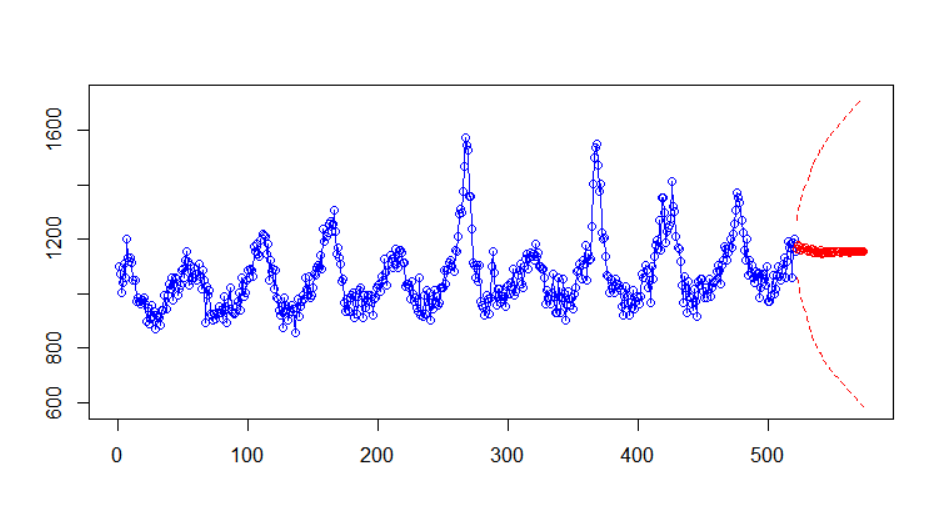
\includegraphics[width=.8\textwidth]{figures/ARAR_test.png}
\caption{ARAR Modelling of Deaths dataset age 65+ from 2010-2019 \cite{deaths_2010-2019}, failing to produce a meaningful forecast.}
\end{figure}
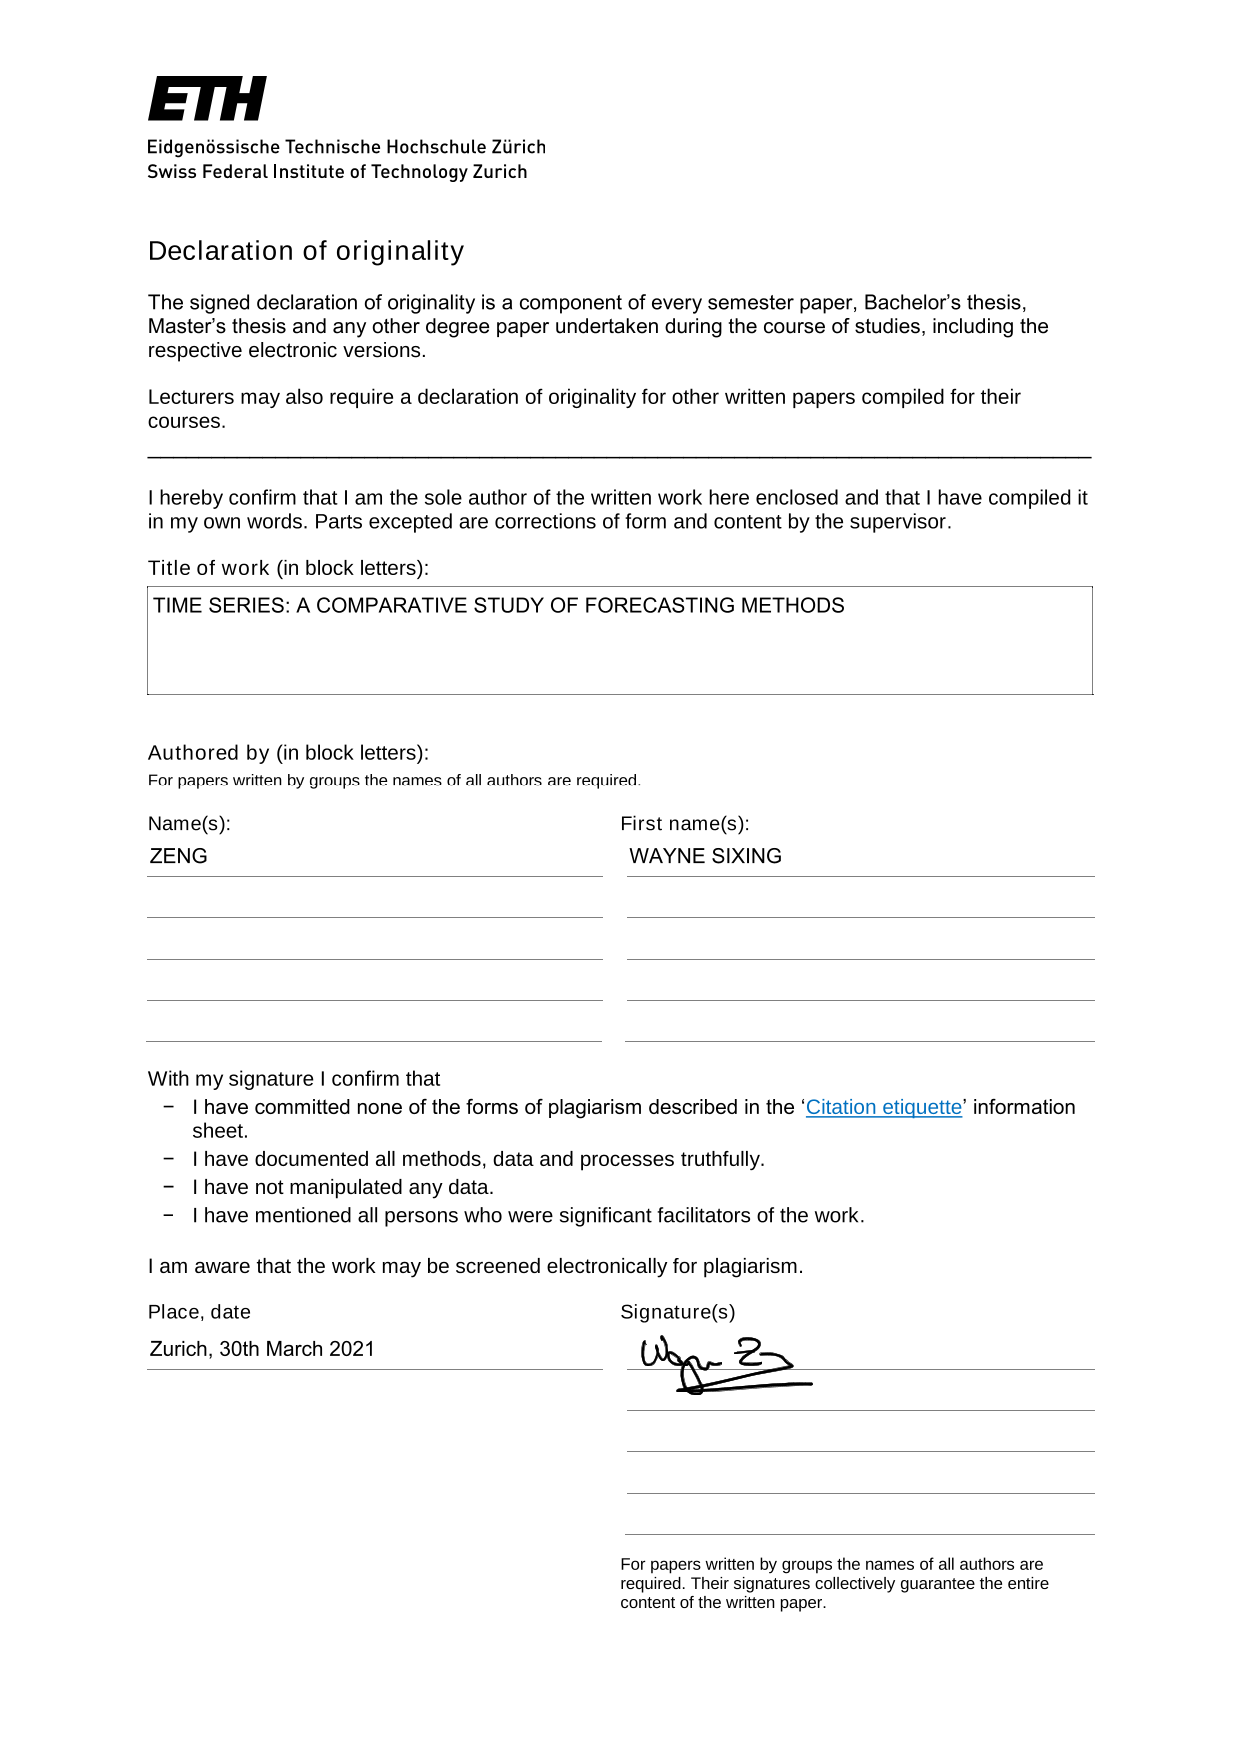
\includepdf[pages=-]{declaration-originality.pdf}
\end{document}